\section{三维连续时间系统:洛伦兹系统}
洛伦兹(Lorenz)系统\cite{lorenz1963deterministic}是1963年由Edward Lorenz提出的描述空气流体运动的一个数学模型。1998年,S.Smale提出21世纪的18个著名的数学问题\cite{smale1998mathematical},其中第14个问题就是关于洛伦兹系统的研究。迄今为止,对洛伦兹系统的研究无论是从数学、物理还是工程上都是十分重要的问题。

\subsection{洛伦兹系统的动力学}
洛伦兹系统的动力学方程\cite{strogatz2001nonlinear}表示为:
\begin{equation}
    \begin{cases}
        \dot{x}=\sigma(y-x)\\
        \dot{y}=x(\rho-z)-y\\
        \dot{z}=xy-\beta z
    \end{cases}\
\end{equation}

该方程描述了一个三维相空间的三个分量对时间的变化率。其中$x$代表对流强度,$y$代表上升流和下降流的温差,$z$代表铅直方向温度分布的非线性强度。$c$是Rayleigh数,为系统的主要控制参数,$a$是Prandt数,$b$是外形比。Lorenz系统具有非线性、非周期性和确定性的性质。参数$\sigma$,$\rho$,$\beta$取不同值时Lorenz系统表现出不同的动力学行为。如在$\rho<1$时,系统只有一个不动点,即原点,所有轨道的长期行为都趋于原点;当$\rho=1$时系统发生了叉式分岔,在$\rho>1$时出现了两个不动点,不动点的稳定性可由其他参数满足的条件确定。三个不动点的坐标分别为$(0,0,0)$、$(\sqrt{\beta(\rho-1)},\sqrt{\beta(\rho-1)},\rho-1)$、$(-\sqrt{\beta(\rho-1)},-\sqrt{\beta(\rho-1)},\rho-1)$。当我们将三个参数取一组特定的值$\rho=28$,$\sigma=10$,$\beta=8/3$时,Lorenz方程的解是混沌的,相空间会存在两个奇异吸引子。

洛伦兹系统的这种动力学特征用传统的非线性动力学知识是比较难分析的,其相图如下:
\begin{figure}
	\centering
	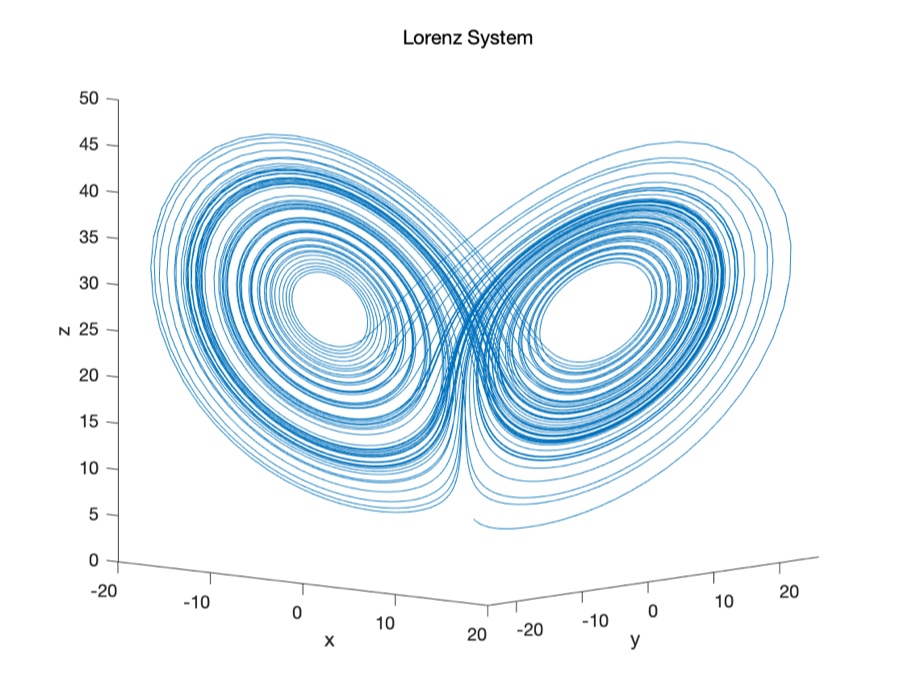
\includegraphics[scale=0.8]{lorenz_phase.png}
    \caption{洛伦兹系统的相图($\rho=28$,$\sigma=10$,$\beta=8/3$)}
    \label{fig:lorz_phas}
\end{figure}
在洛伦兹系统中,所有的非平衡解最终趋向同一个复杂的集合,这就是所谓的洛伦兹吸引子\cite{lorenz1963deterministic}。我们将在取上述参数的条件下,通过Lorenz微分方程演化出相空间的一条轨道,作为Koopman分析的源数据,以此来分析Lorenz系统的特征。

\subsection{洛伦兹系统的Koopman算符本征函数}
我们已经探究了帐篷映射、Logistic映射、埃农映射系统中Koopman算符的本征值与本征函数。洛伦兹系统是一个三维流系统,在三维流系统中Koopman算符的本征函数的计算又稍有区别,三维流系统中还涉及到时间维度的动力学,且动力学特征也更为复杂。在本节中,我们将探究Koopman算符的本征值与本征函数与洛伦兹系统的动力学特征的关系。

\subsubsection{正交完备基函数空间}
洛伦兹系统是一个三维流系统,在三维函数空间中,三维高斯基函数可以写为
\begin{equation}
  g(x,y)=Ce^{({\dfrac{-(x-x_j)^2-(y-y_j)^2-(z-z_j)^2}{d_j^2}})}
\end{equation}
其中C为常系数,$(x_j,y_j,z_j)$为高斯波包的中心位置,$d_j$表示格点宽度,且我们在两个方向上并无相关性。

我们将某一时刻的二维数据矩阵作为一组状态变量,并求得每个基函数在此状态变量下的值,作为数据矩阵,以此求得演化前矩阵$K$,经过一个微笑的时间$t=0.001s$演化后,我们得到演化之后的数据矩阵,并计算每个基函数在此状态变量下的值,以此求得演化后矩阵$L$。根据式\eqref{eq:Koop_kl1},计算Koopman算符$U$的矩阵表示及其本征值与本征函数。

图\ref{fig:lorenz_eig_gauss}画出了演化格点数量$n=10000$,在三维高斯基函数下洛伦兹系统的本征值和本征函数,其中数据矩阵$K$与演化后数据矩阵$L$的时间间隔$t=0.001s$,高斯基函数数量$m=8\times 12\times 10$,格点宽度$d_j=5$。我们取相空间$[-20,20]\times [-20,20]\times [0,50]$,并取前9个本征值接近1对应的本征函数,当本征函数为复数时,我们取实部作为我们的本征函数。同时,我们分布画出了本征函数的实部、虚部、模、幅角。
\begin{figure}
    \centering
    \subfloat[实部]{
      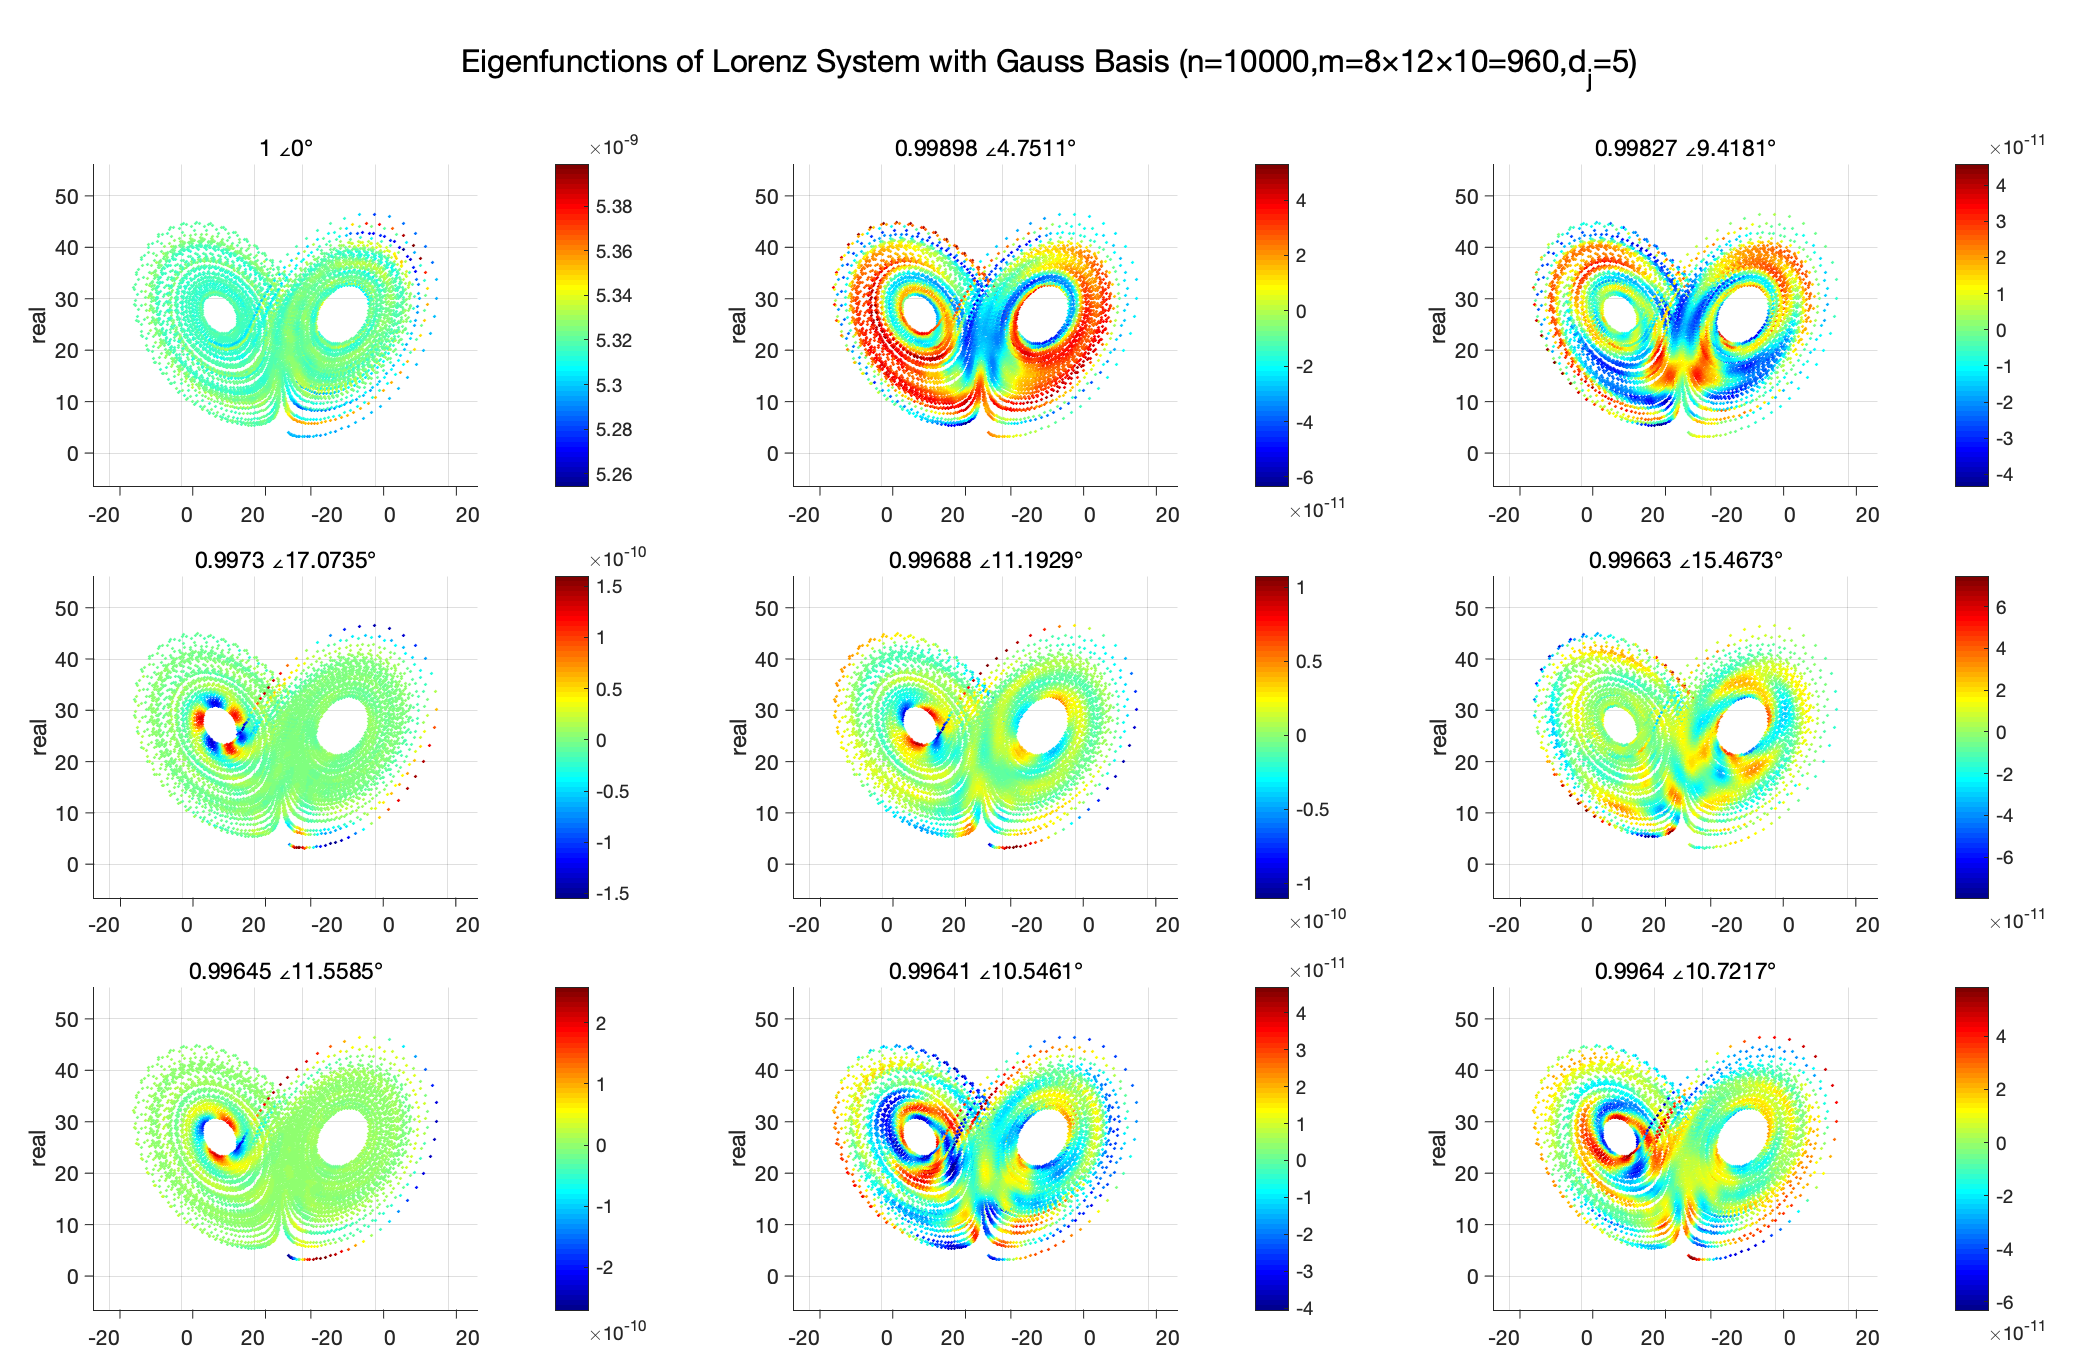
\includegraphics[scale=0.2]{lorenz/Lorenz_eigen_Gauss_leftU_real_n10000m960}}
    \subfloat[虚部]{
      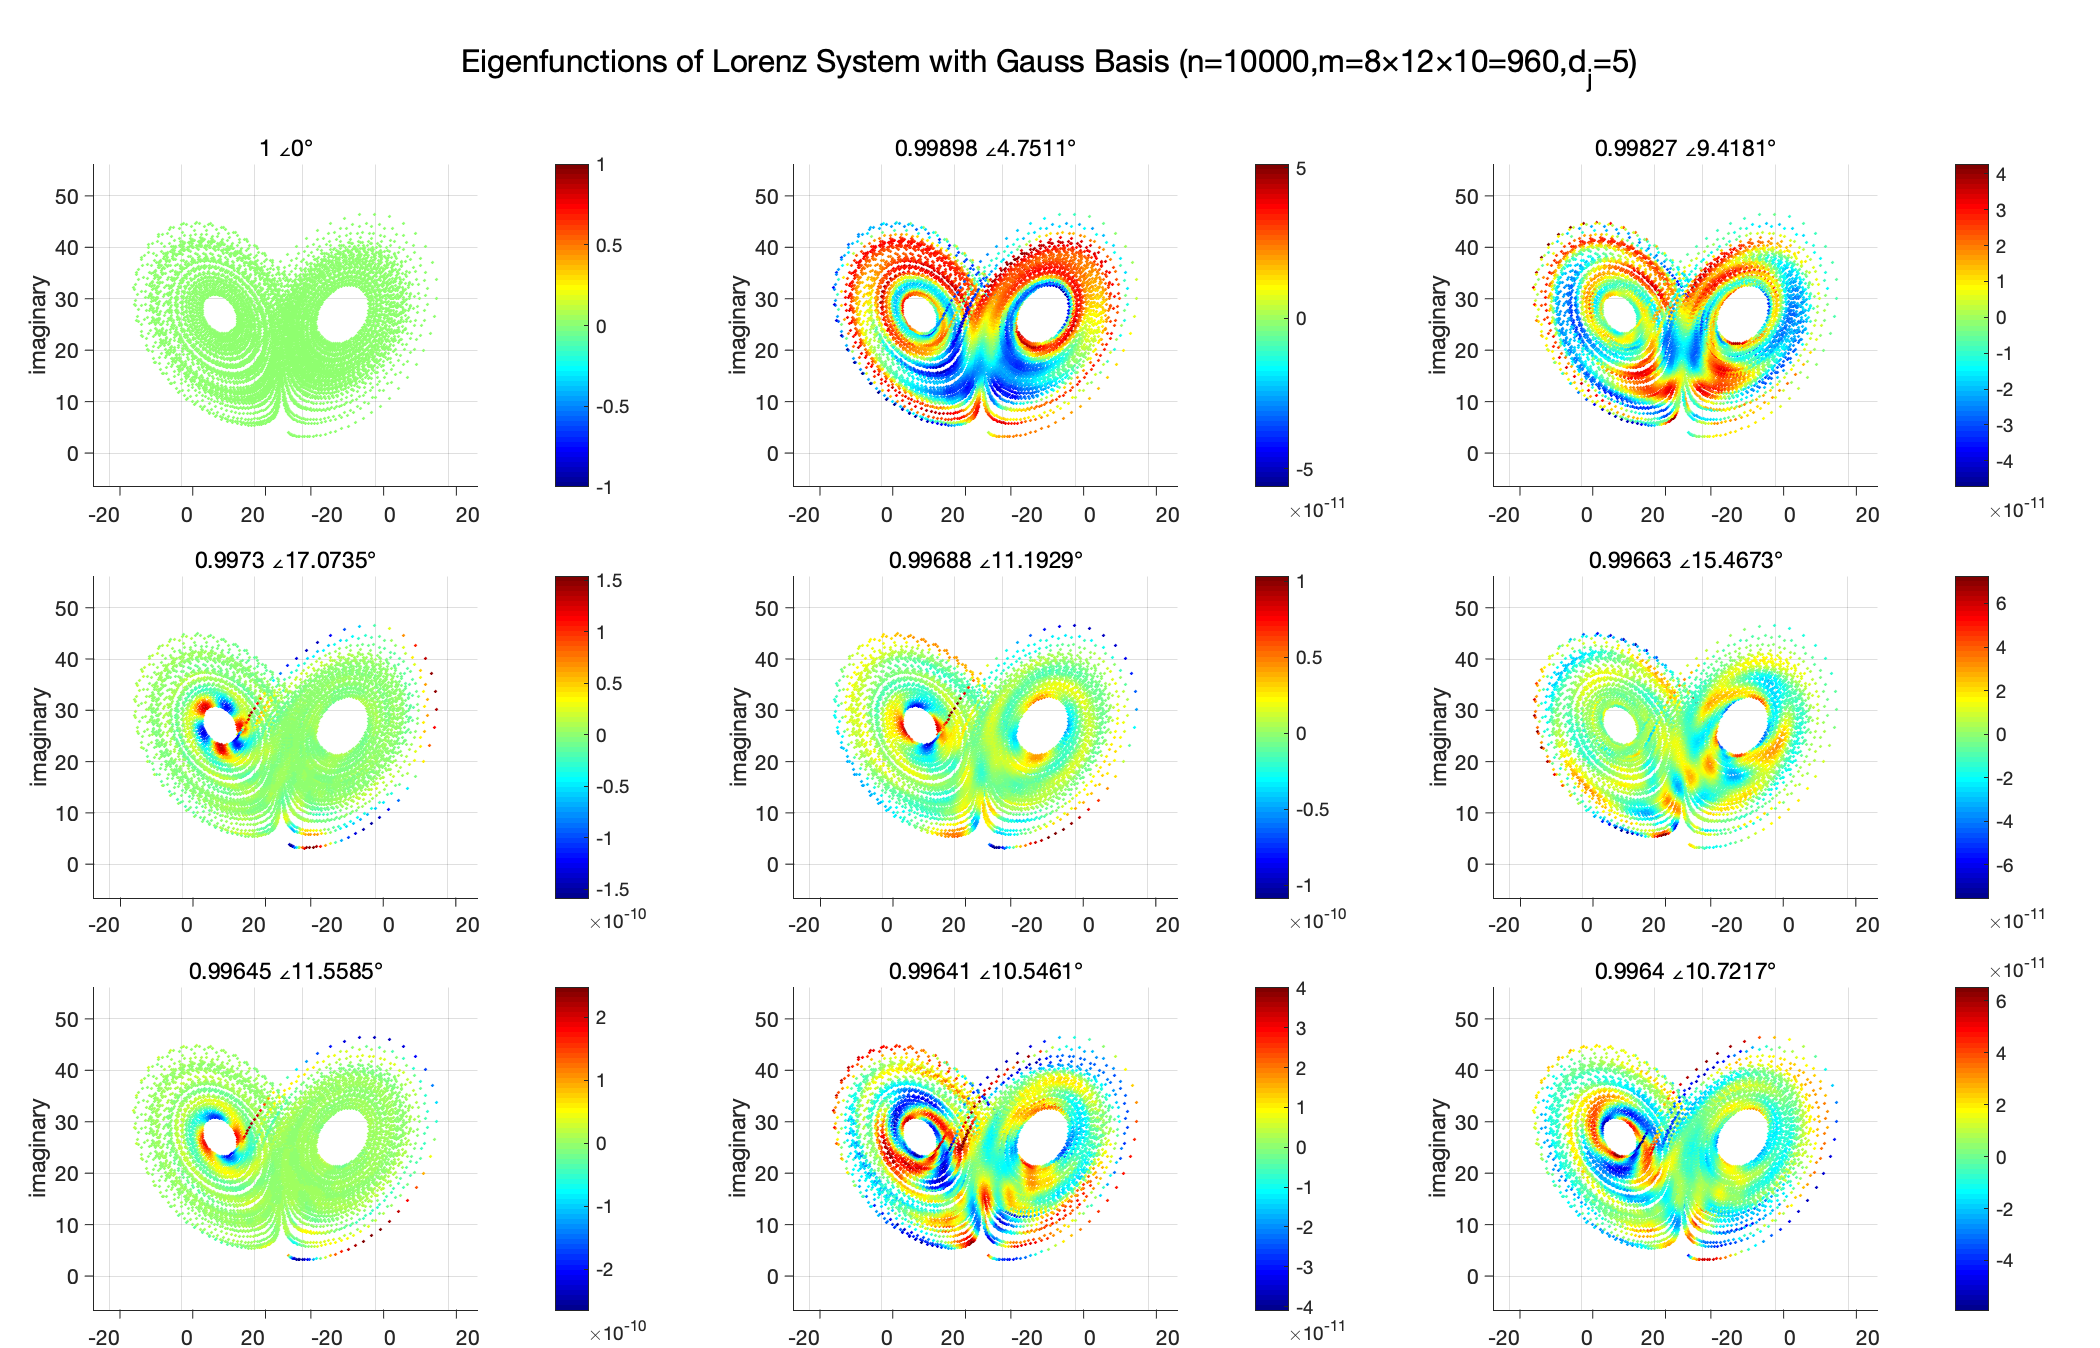
\includegraphics[scale=0.2]{lorenz/Lorenz_eigen_Gauss_leftU_imag_n10000m960}}
    \\
    \subfloat[模]{
      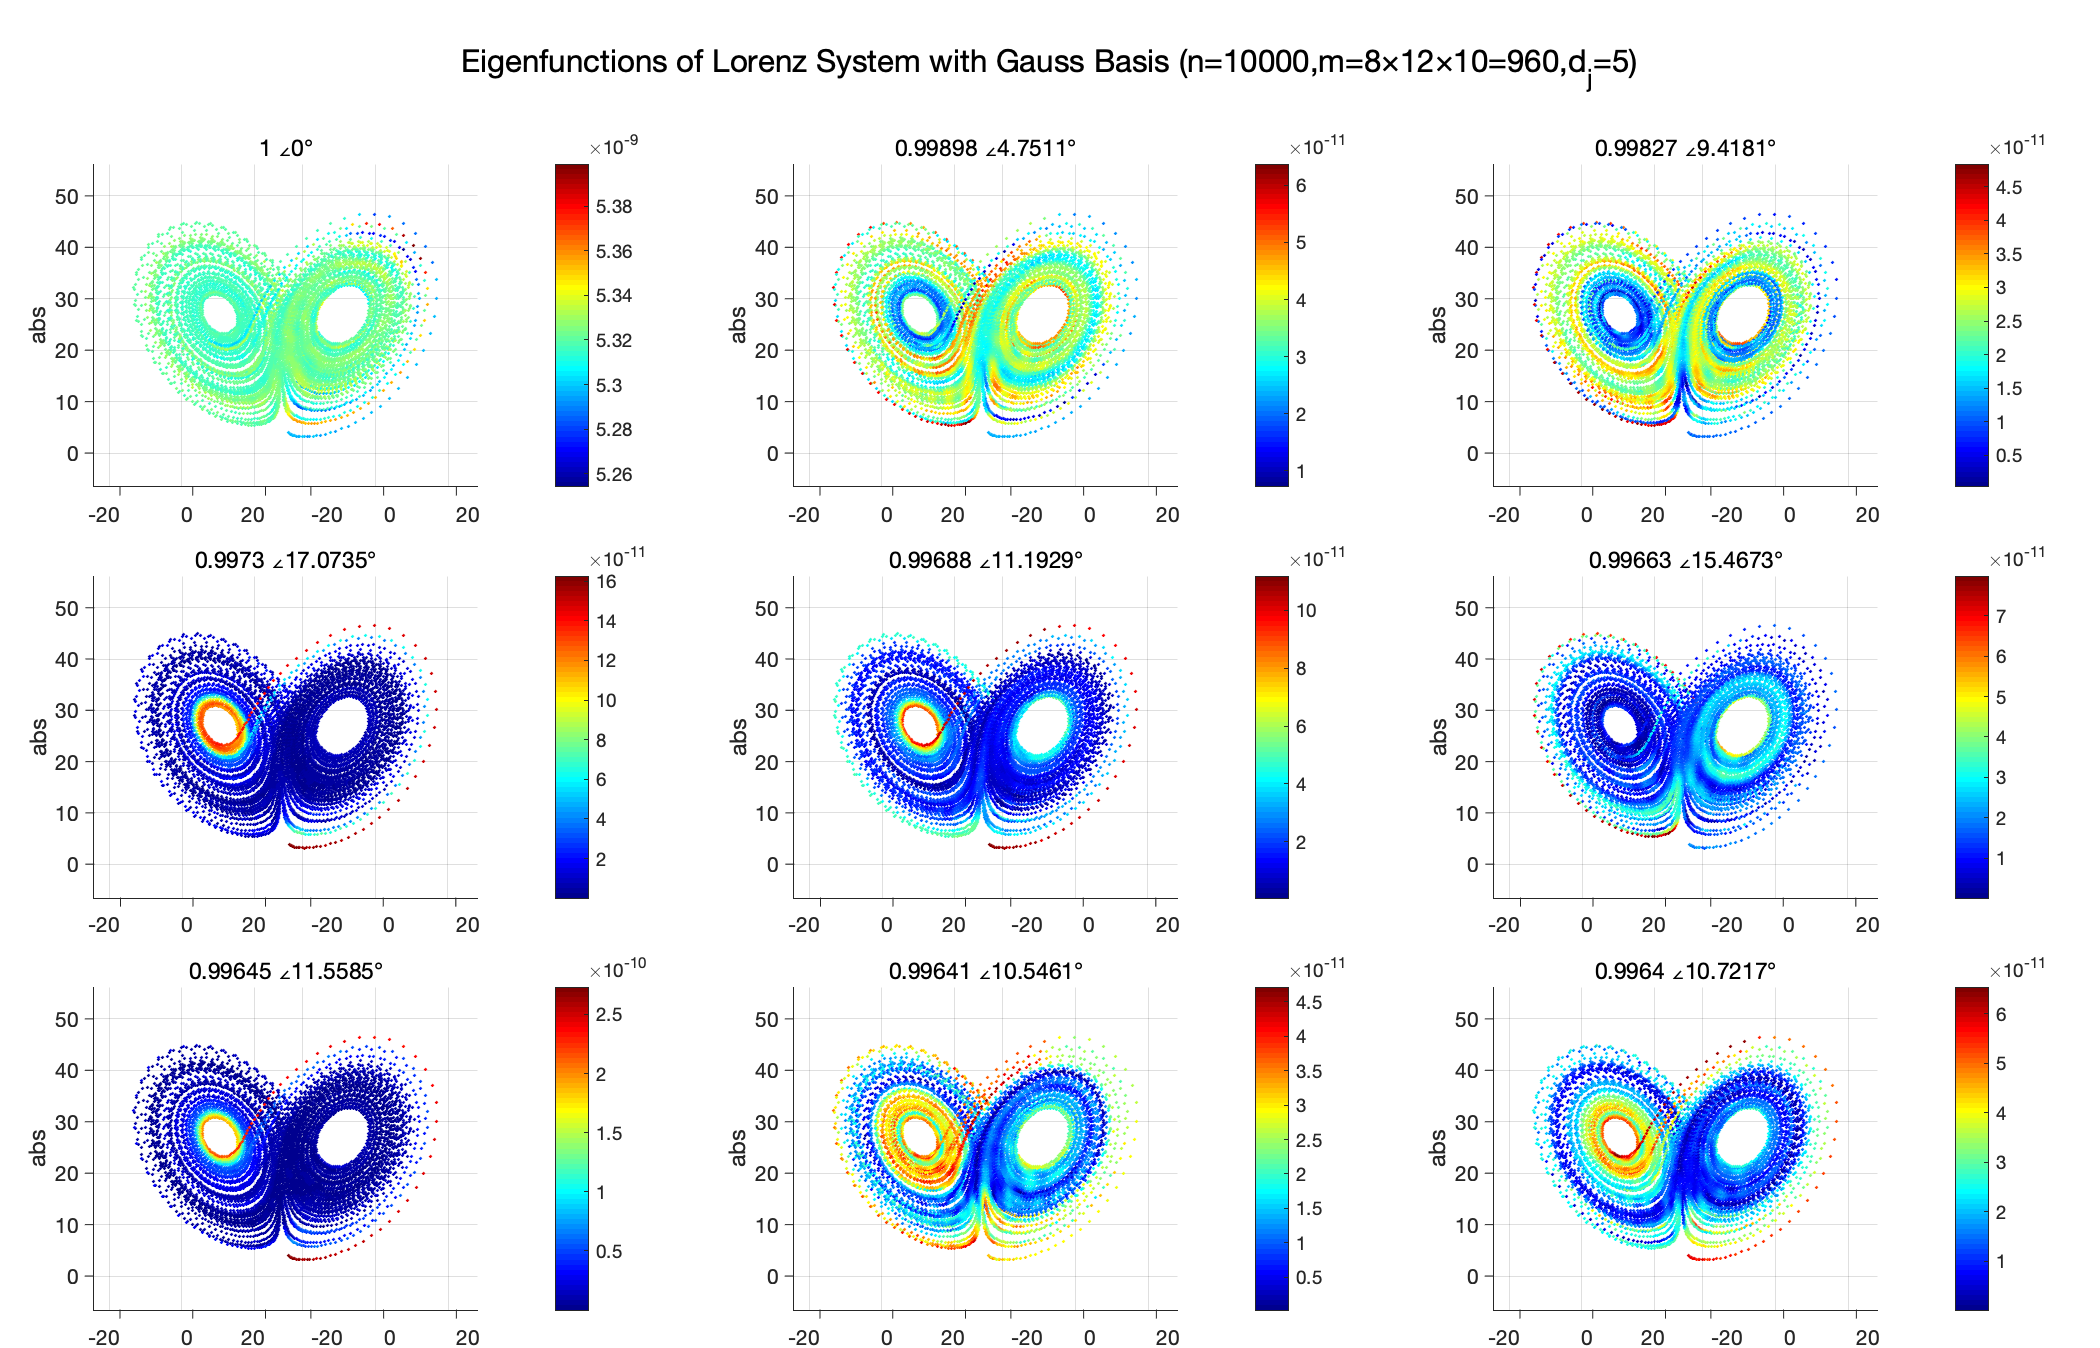
\includegraphics[scale=0.2]{lorenz/Lorenz_eigen_Gauss_leftU_abs_n10000m960}}
    \subfloat[幅角]{
      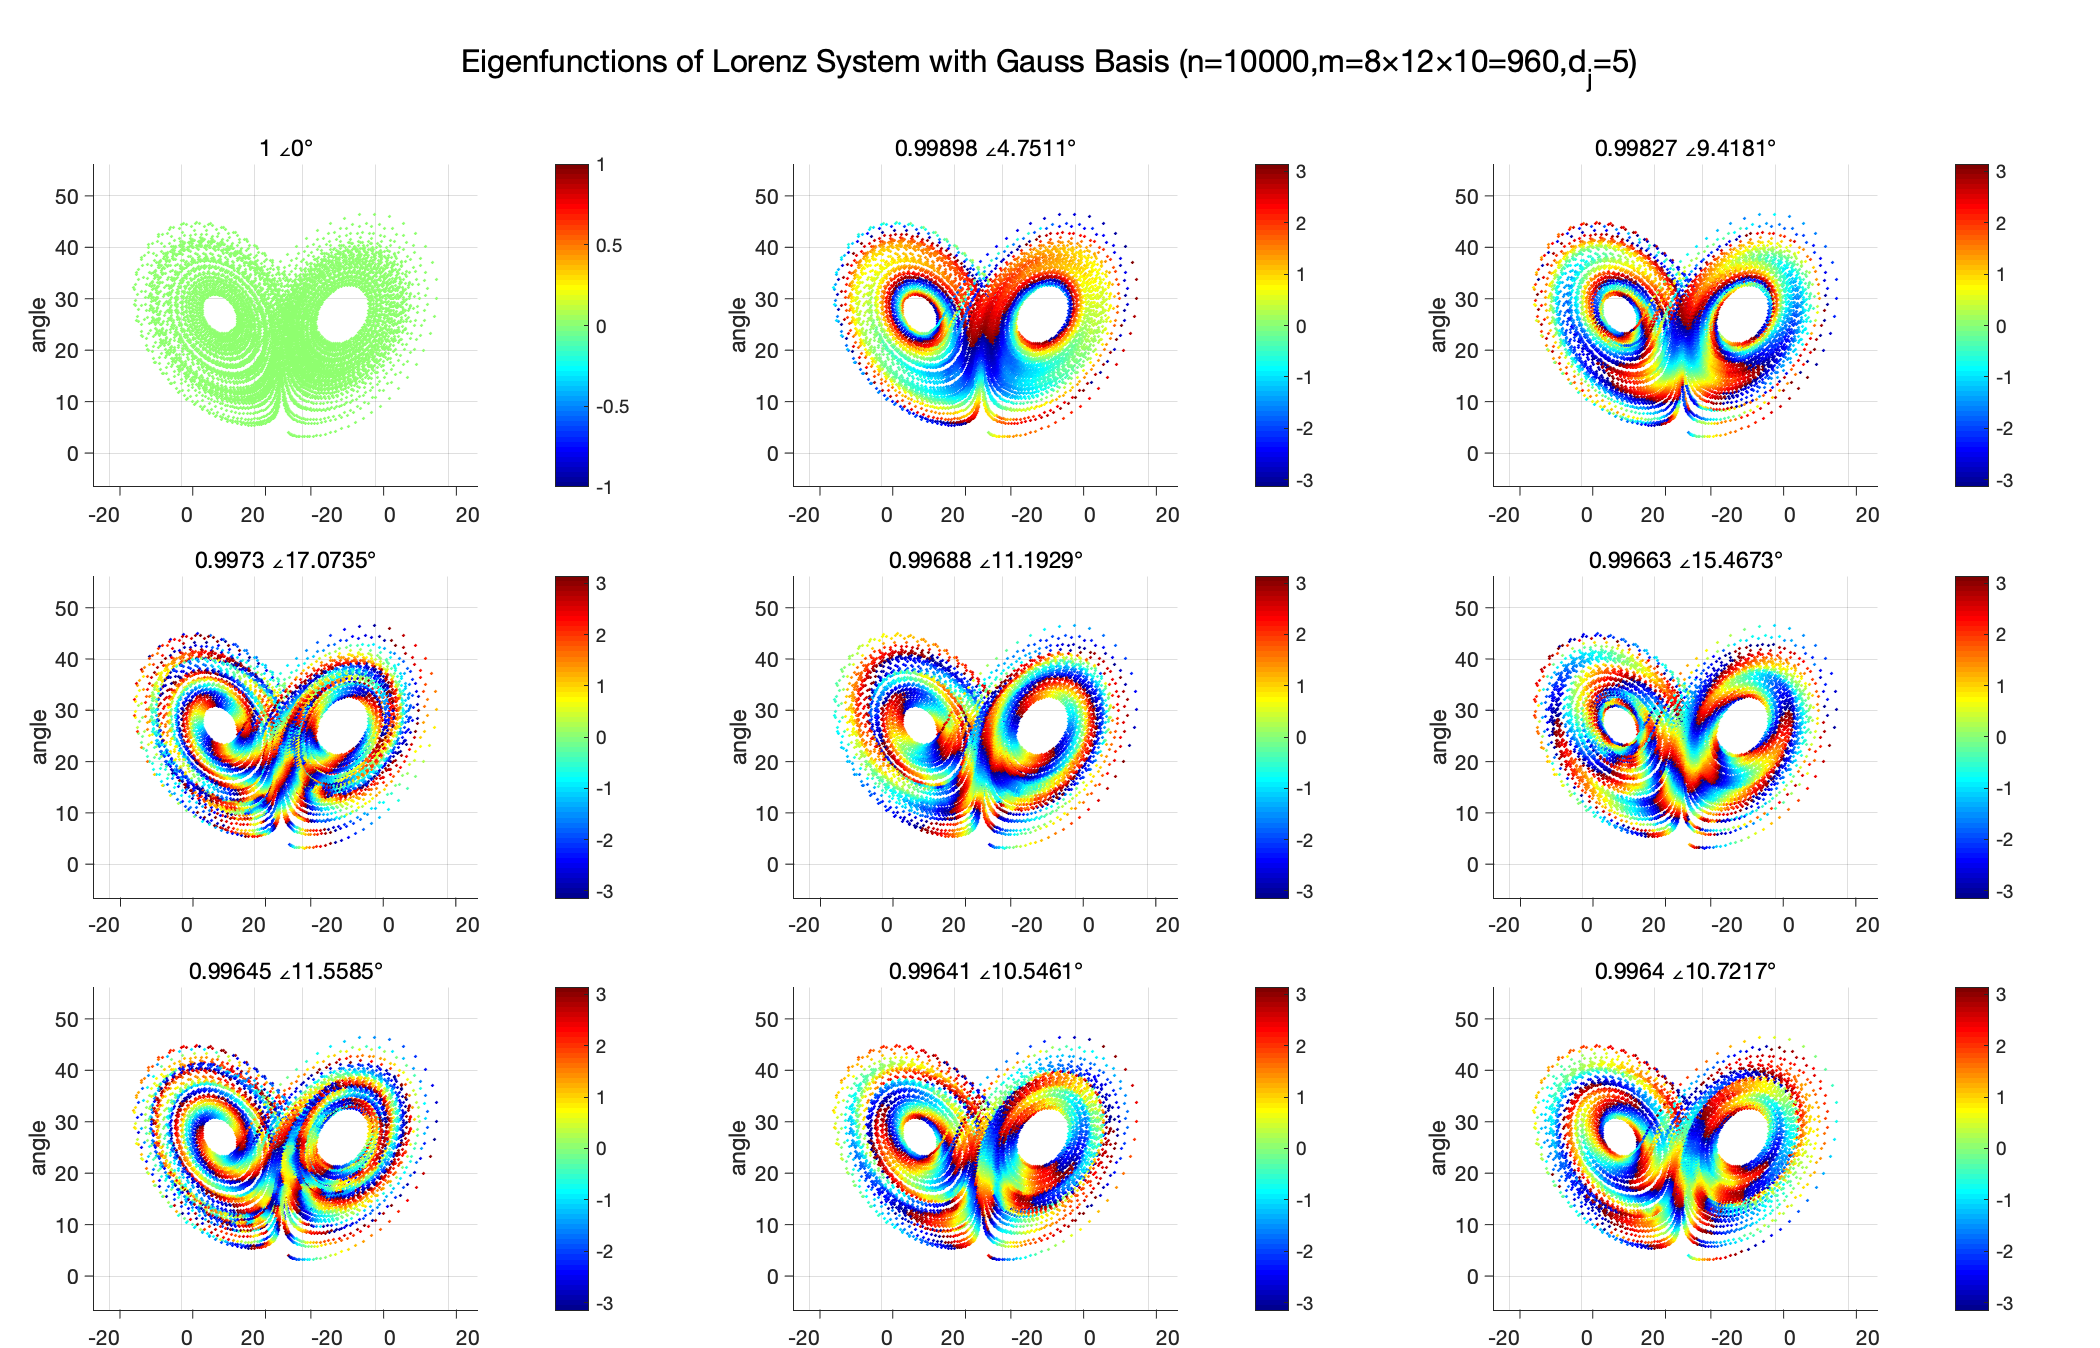
\includegraphics[scale=0.2]{lorenz/Lorenz_eigen_Gauss_leftU_angle_n10000m960}}
    \\
    \caption{洛伦兹系统三维高斯基的本征函数($n=10000,m=960$)}\label{fig:lorenz_eig_gauss}
\end{figure}

从图\ref{fig:lorenz_eig_gauss}中,我们发现在高斯基函数下,洛伦兹系统的吸引子随着时间演化在本征函数中有着一定分布,且本征函数值的不同将洛伦兹吸引子划分出不同区域,如在图\ref{fig:lorenz_eig_gauss}实部的第2张子图中,随着时间的演化,洛伦兹系统在每圈演化中分别经历了蓝色和红色的本征值,具有近似的周期行为。若我们关心最关键的分隔区域,我们可以考虑观察洛伦兹系统的本征函数的幅角,因为幅角可以将本征函数值限定在$[-180°,180°]$,我们通过观察幅角的正负来将吸引子划分为两个动力学性质不同的区域。图\ref{fig:lorenz_eig_gauss_angle}画出了根据本征函数幅角的正负将吸引子区域划分的结果。

\begin{figure}
	\centering
	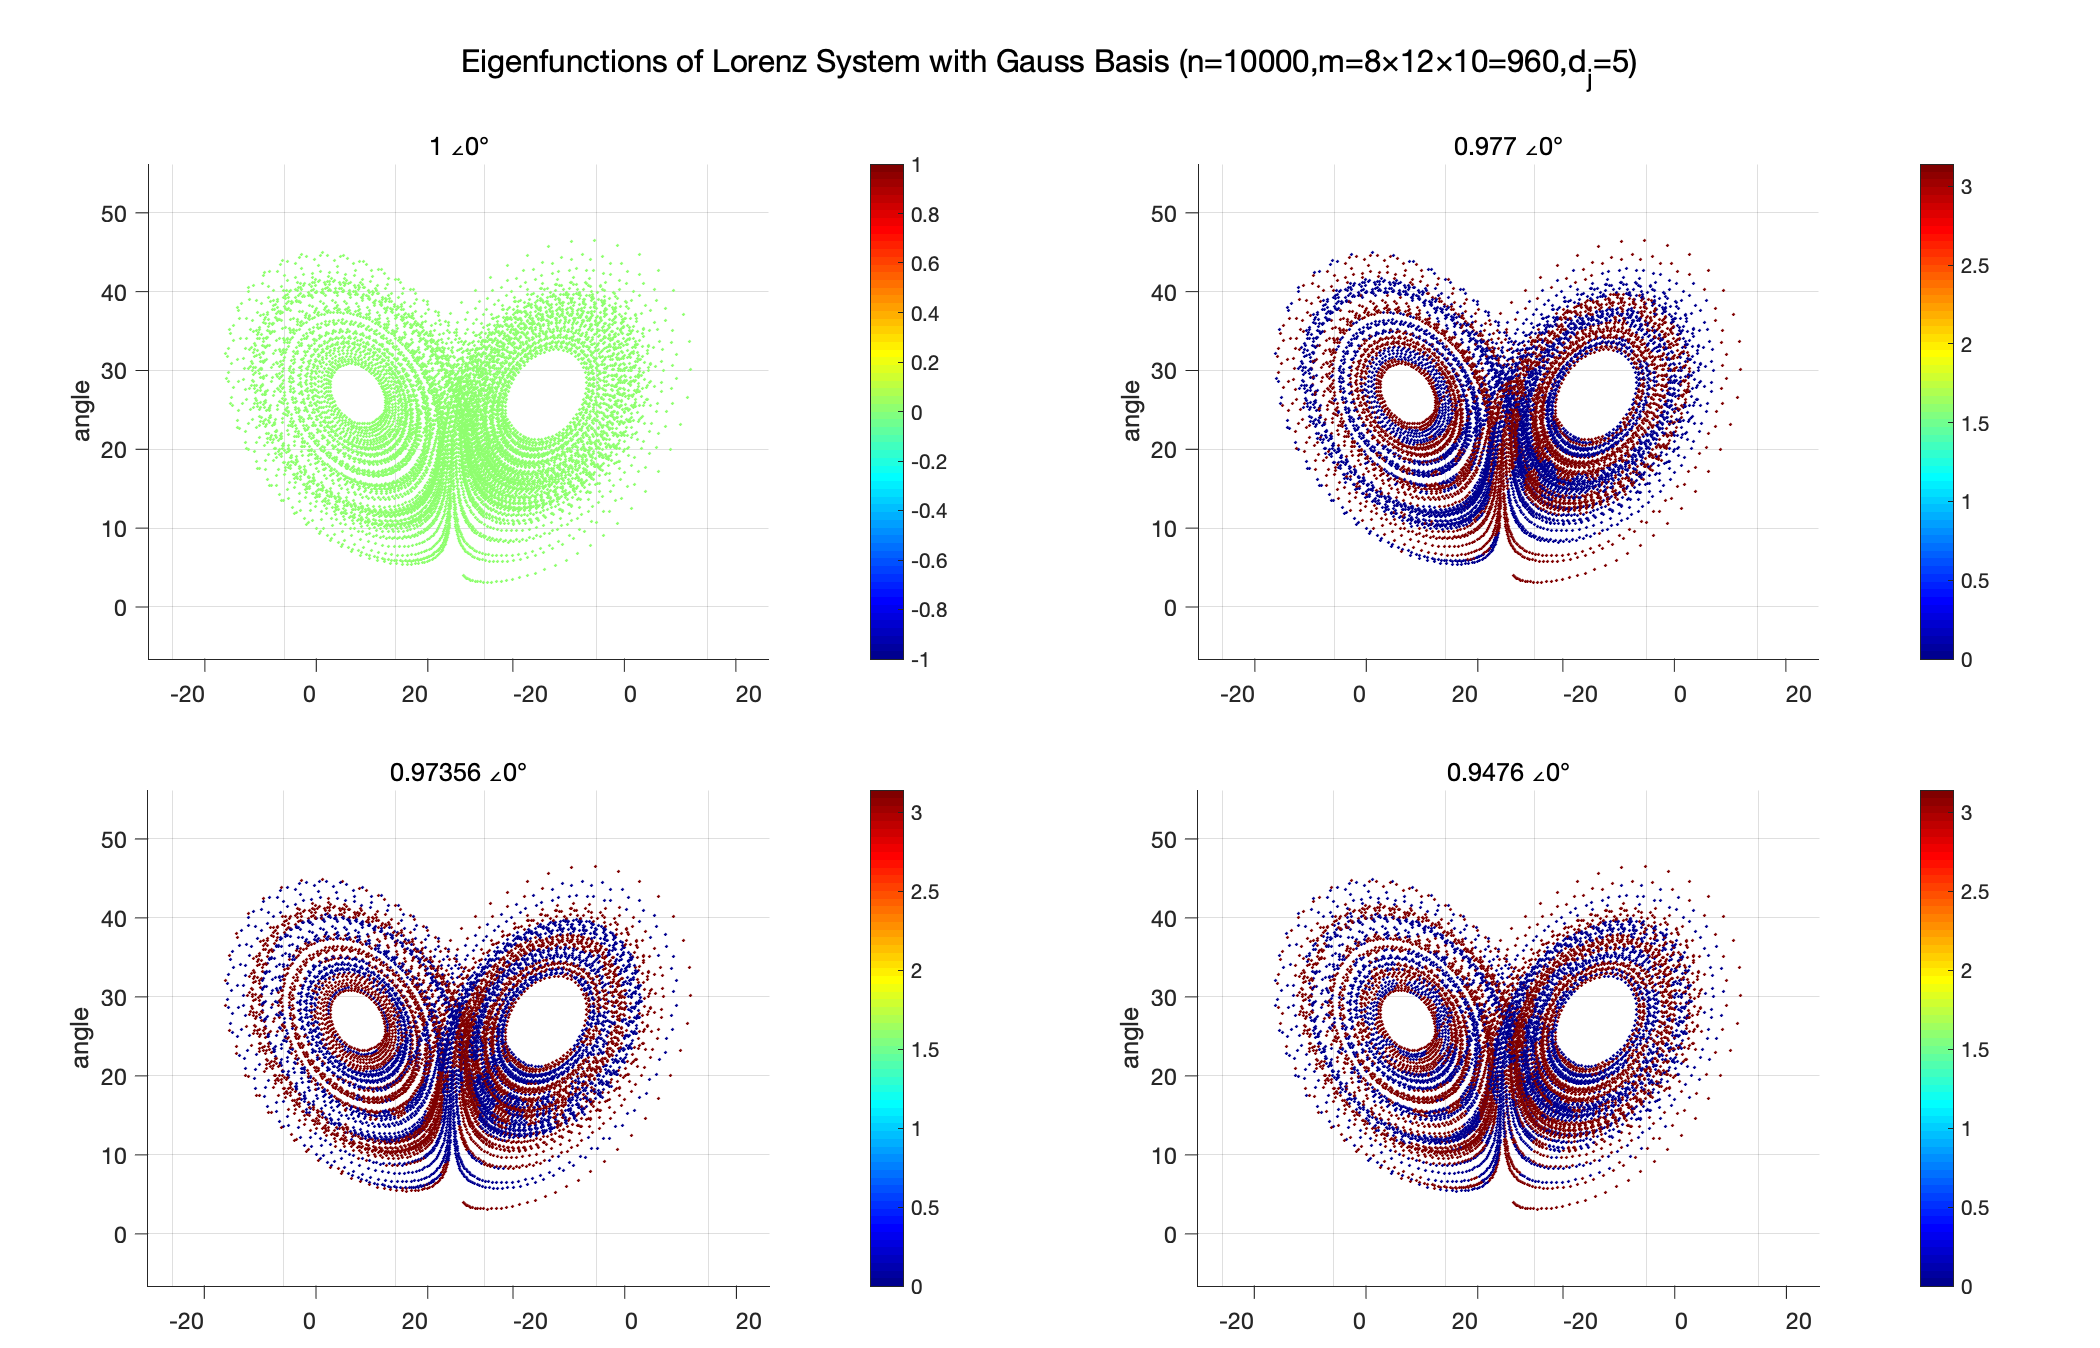
\includegraphics[scale=0.4]{lorenz/Lorenz_eigen_Gauss_leftU_realL_n10000m960}
    \caption{洛伦兹系统三维高斯基的本征函数(幅角)($n=10000,m=960$)}\label{fig:lorenz_eig_gauss_angle}
\end{figure}

在图\ref{fig:lorenz_eig_gauss_angle}中,我们选取了4个实本征值对应的本征函数,并取本征函数的幅角作图,图中可以看出红色区域和蓝色区域将洛伦兹系统的吸引子分成了两块不同的区域,在之前的讨论中,我们认为本征值接近1的本征函数反映了相空间中一条随时间演化不变的轨道,我们可以认为我们划分的两个区域属于洛伦兹系统的一个不变集\cite{brunton2016koopman},而这种不变集可能就对应洛伦兹系统的周期轨道。

\subsubsection{自然基函数空间}
在式\eqref{eq:Koop_kl2}中,我们可以通过构造自然函数格点来计算Koopman算符的本征值与本征函数,洛伦兹系统是一个三维流系统,其存在三个维度,每个维度都可以作为一组自然基函数,于是我们在吸引子区域分别画出了三个维度的自然基函数空间下的本征函数,并分别取本征的实部与模作图。

图\ref{fig:lorenz_eig_natural}画出了在演化格点数量$n=10000$,基函数数量$m=4$时,不同本征值下洛伦兹系统在吸引子域上的本征函数图像,每个子图都画了三个维度的本征函数,其中第一行表示本征函数的实部,第二行表示本征函数的模。
\begin{figure}
    \centering
    \subfloat{
      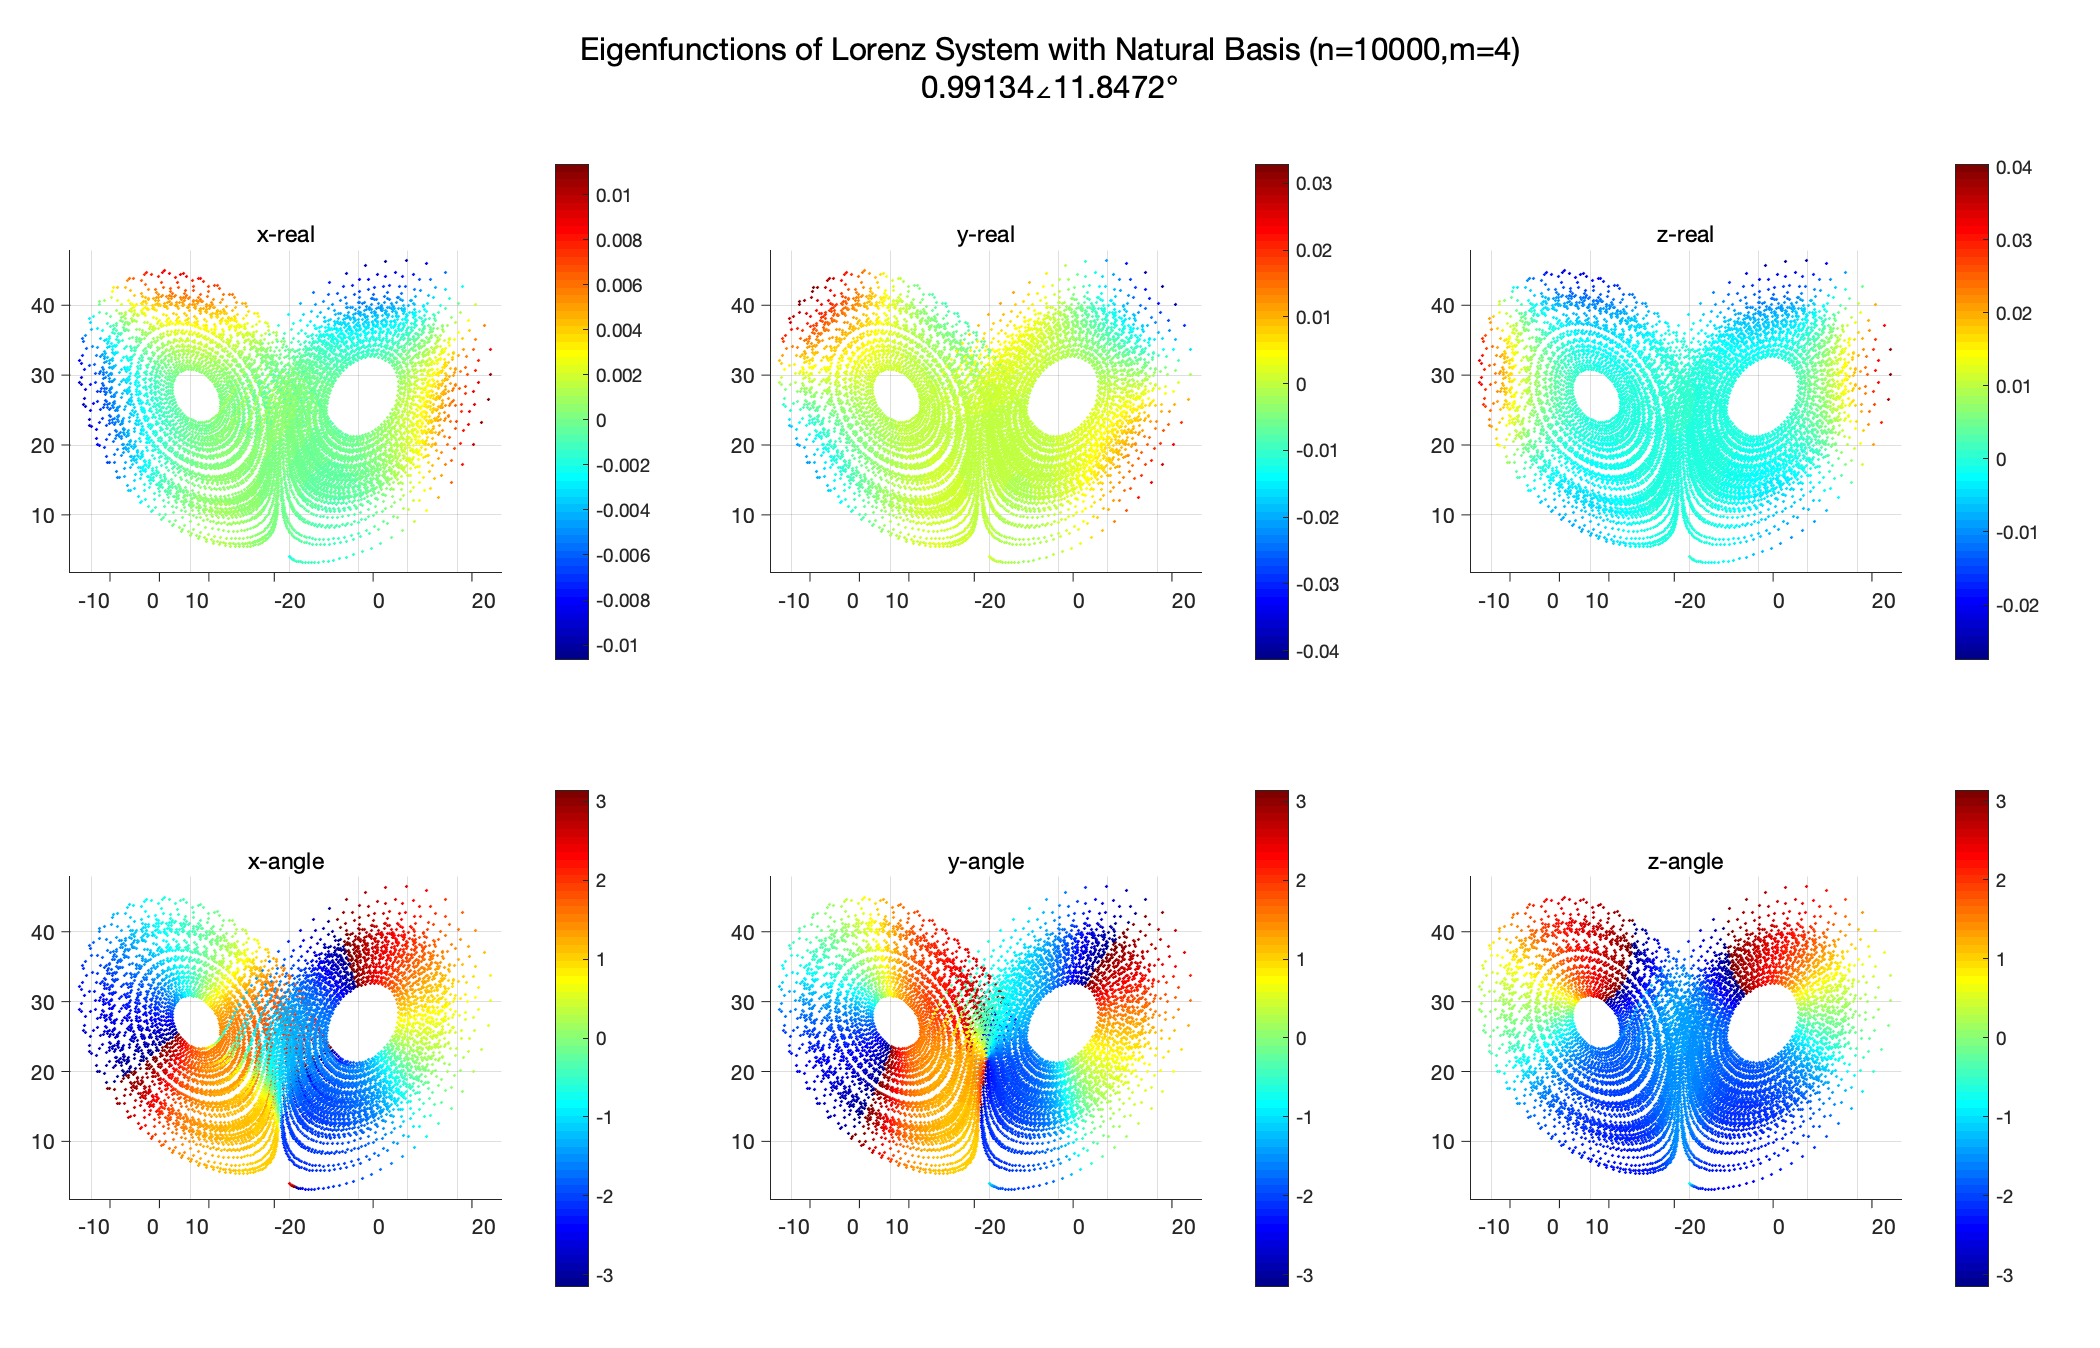
\includegraphics[scale=0.2]{lorenz/natural/Lorenz_eigen_natural_n10000m4figure1}}
    \subfloat{
      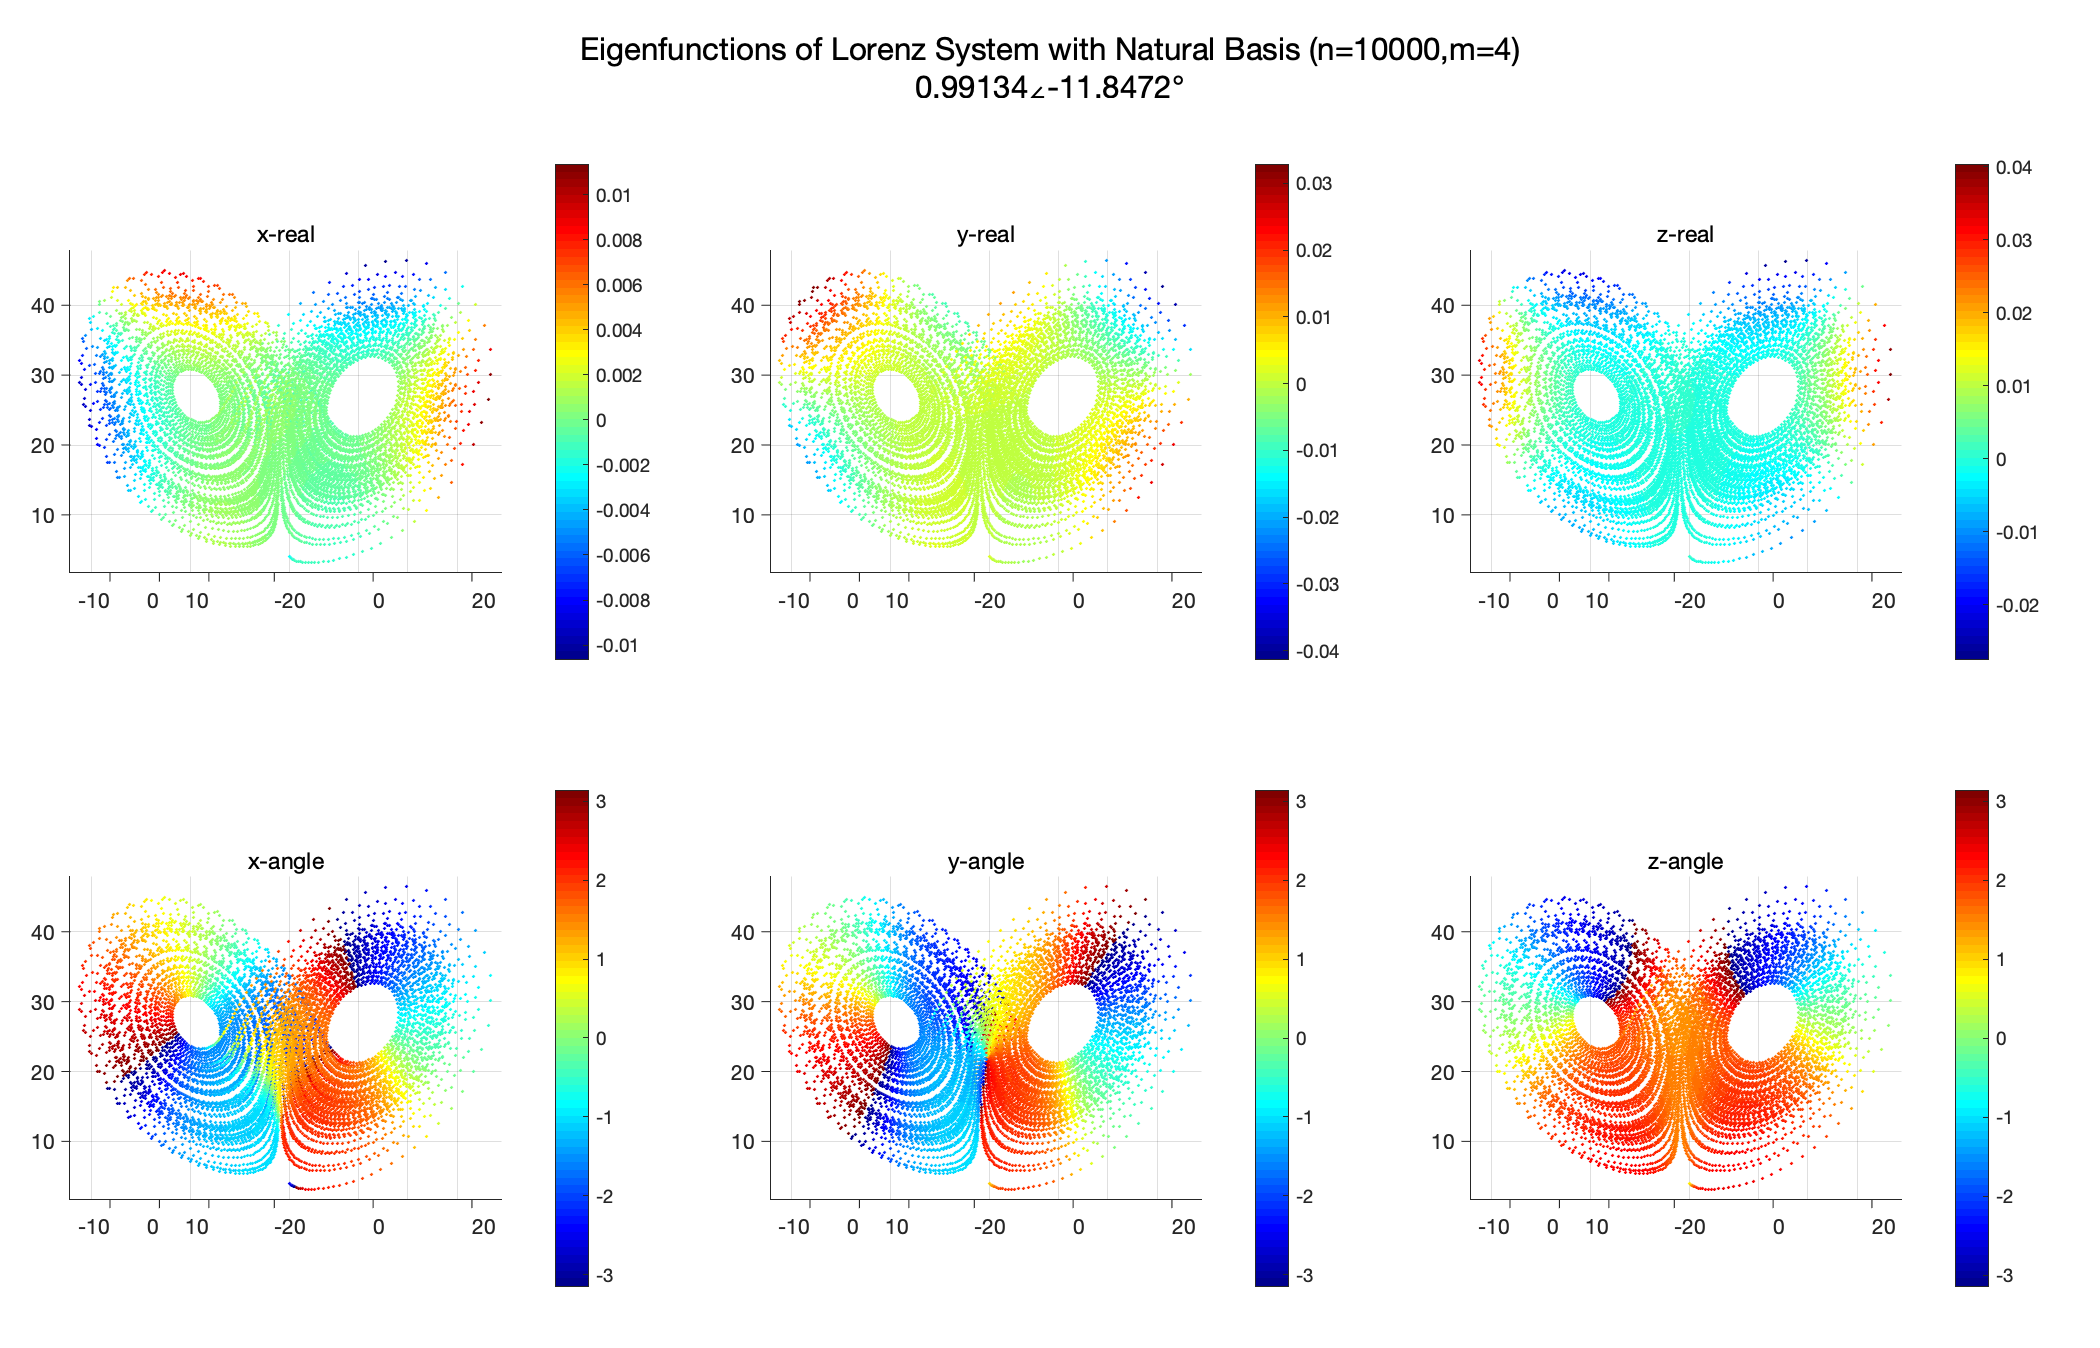
\includegraphics[scale=0.2]{lorenz/natural/Lorenz_eigen_natural_n10000m4figure2}}
    \\
    \subfloat{
      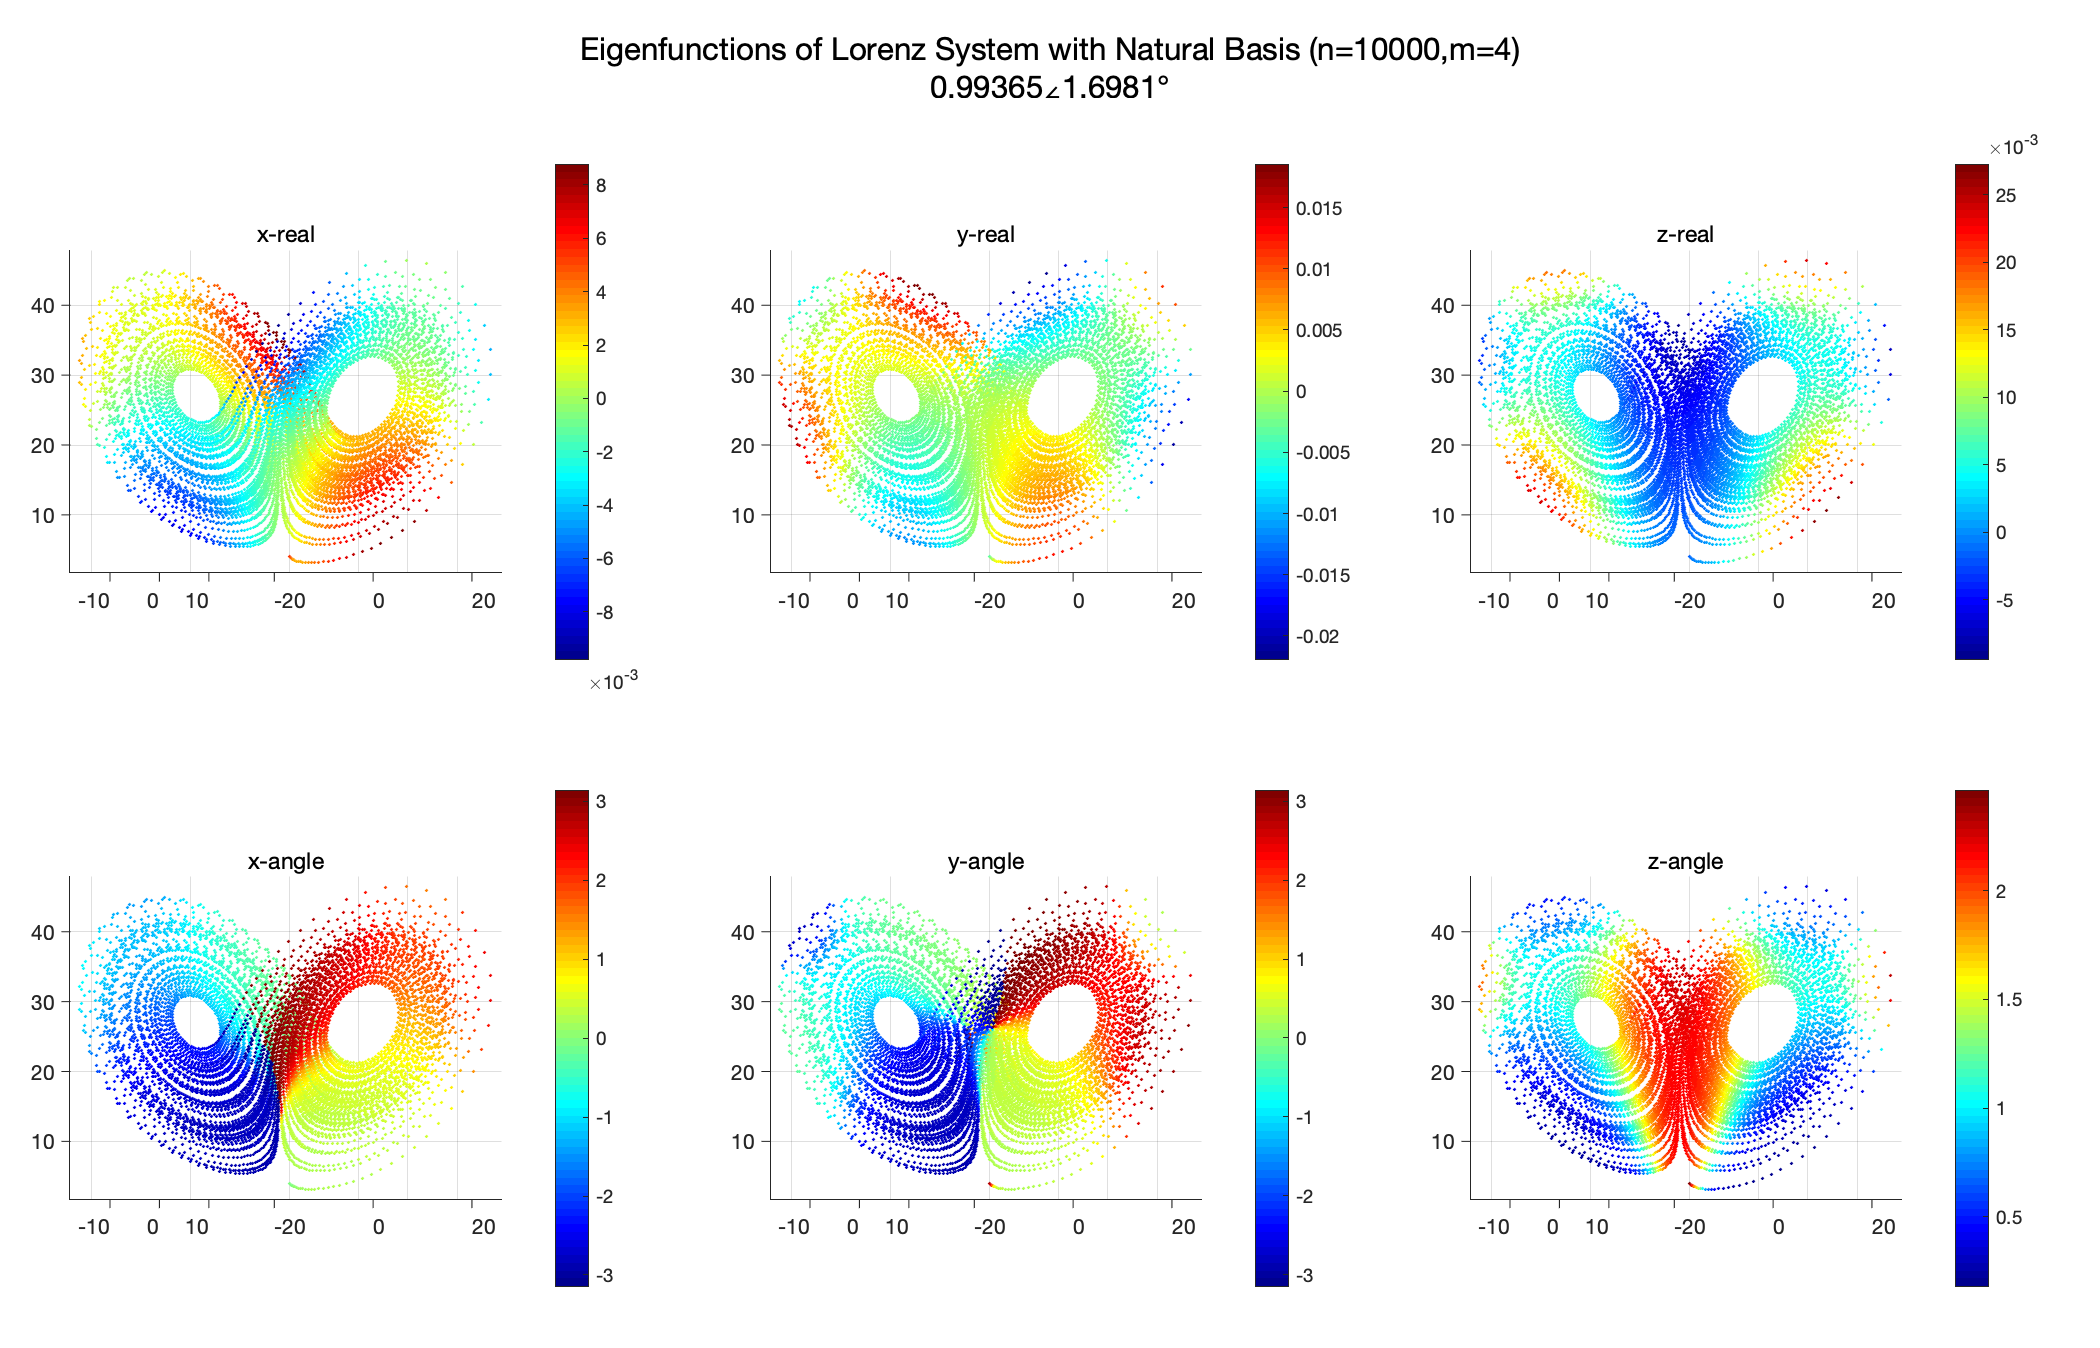
\includegraphics[scale=0.2]{lorenz/natural/Lorenz_eigen_natural_n10000m4figure3}}
    \subfloat{
      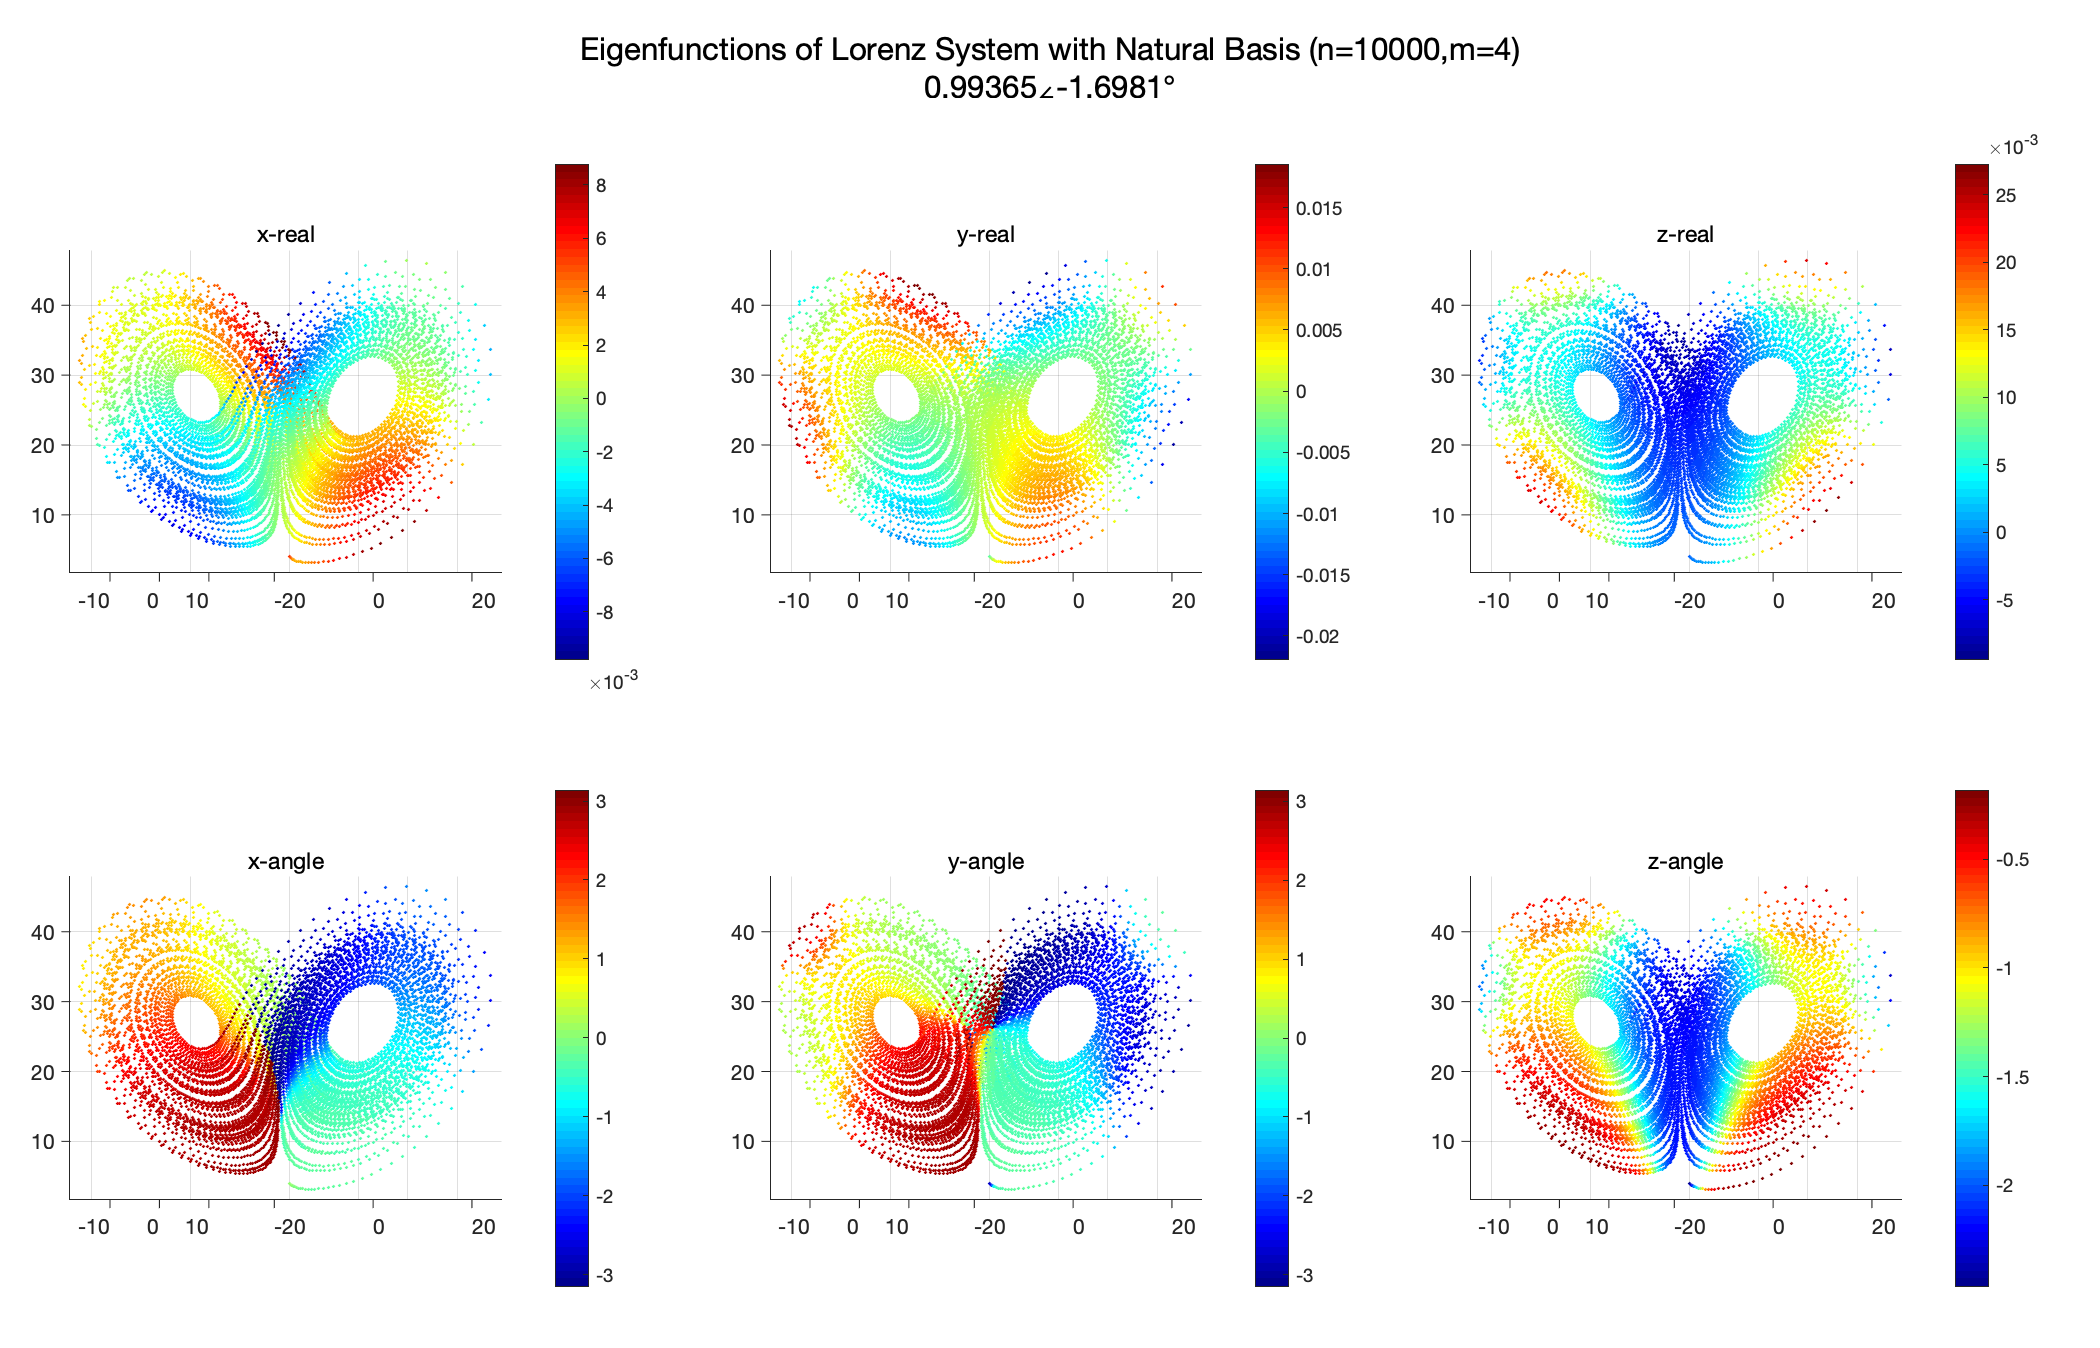
\includegraphics[scale=0.2]{lorenz/natural/Lorenz_eigen_natural_n10000m4figure4}}
    \\
    \caption{洛伦兹系统自然基下的本征函数($n=10000,m=4$):每个子图表示不同本征值下的自然基函数本征函数图像,其中每个子图又分为六个小图,其中第一行表示本征函数的实部,第二行表示本征函数的模}\label{fig:lorenz_eig_natural}
\end{figure}

图\ref{fig:lorenz_eig_natural}中我们可以看出在自然基函数下,本征函数展示出了倍频特征,随着时间的演化,本征函数在每圈吸引子的演化中有着近似周期性的规律,为了更清晰的揭示这种规律,我们画出在不同基函数$m$下的本征函数,以此来探究自然基函数中基函数个数对本征函数的影响。

图\ref{fig:lorenz_eig_natural_real}画出了在演化格点$n=10000$,基函数数量$m=1,2,3,4,5,6,7,8$,计算$x$维度本征函数的实部,不同本征值下洛伦兹系统在吸引子域上的本征函数图像。

\begin{figure}
    \centering
    \subfloat[m=1]{
      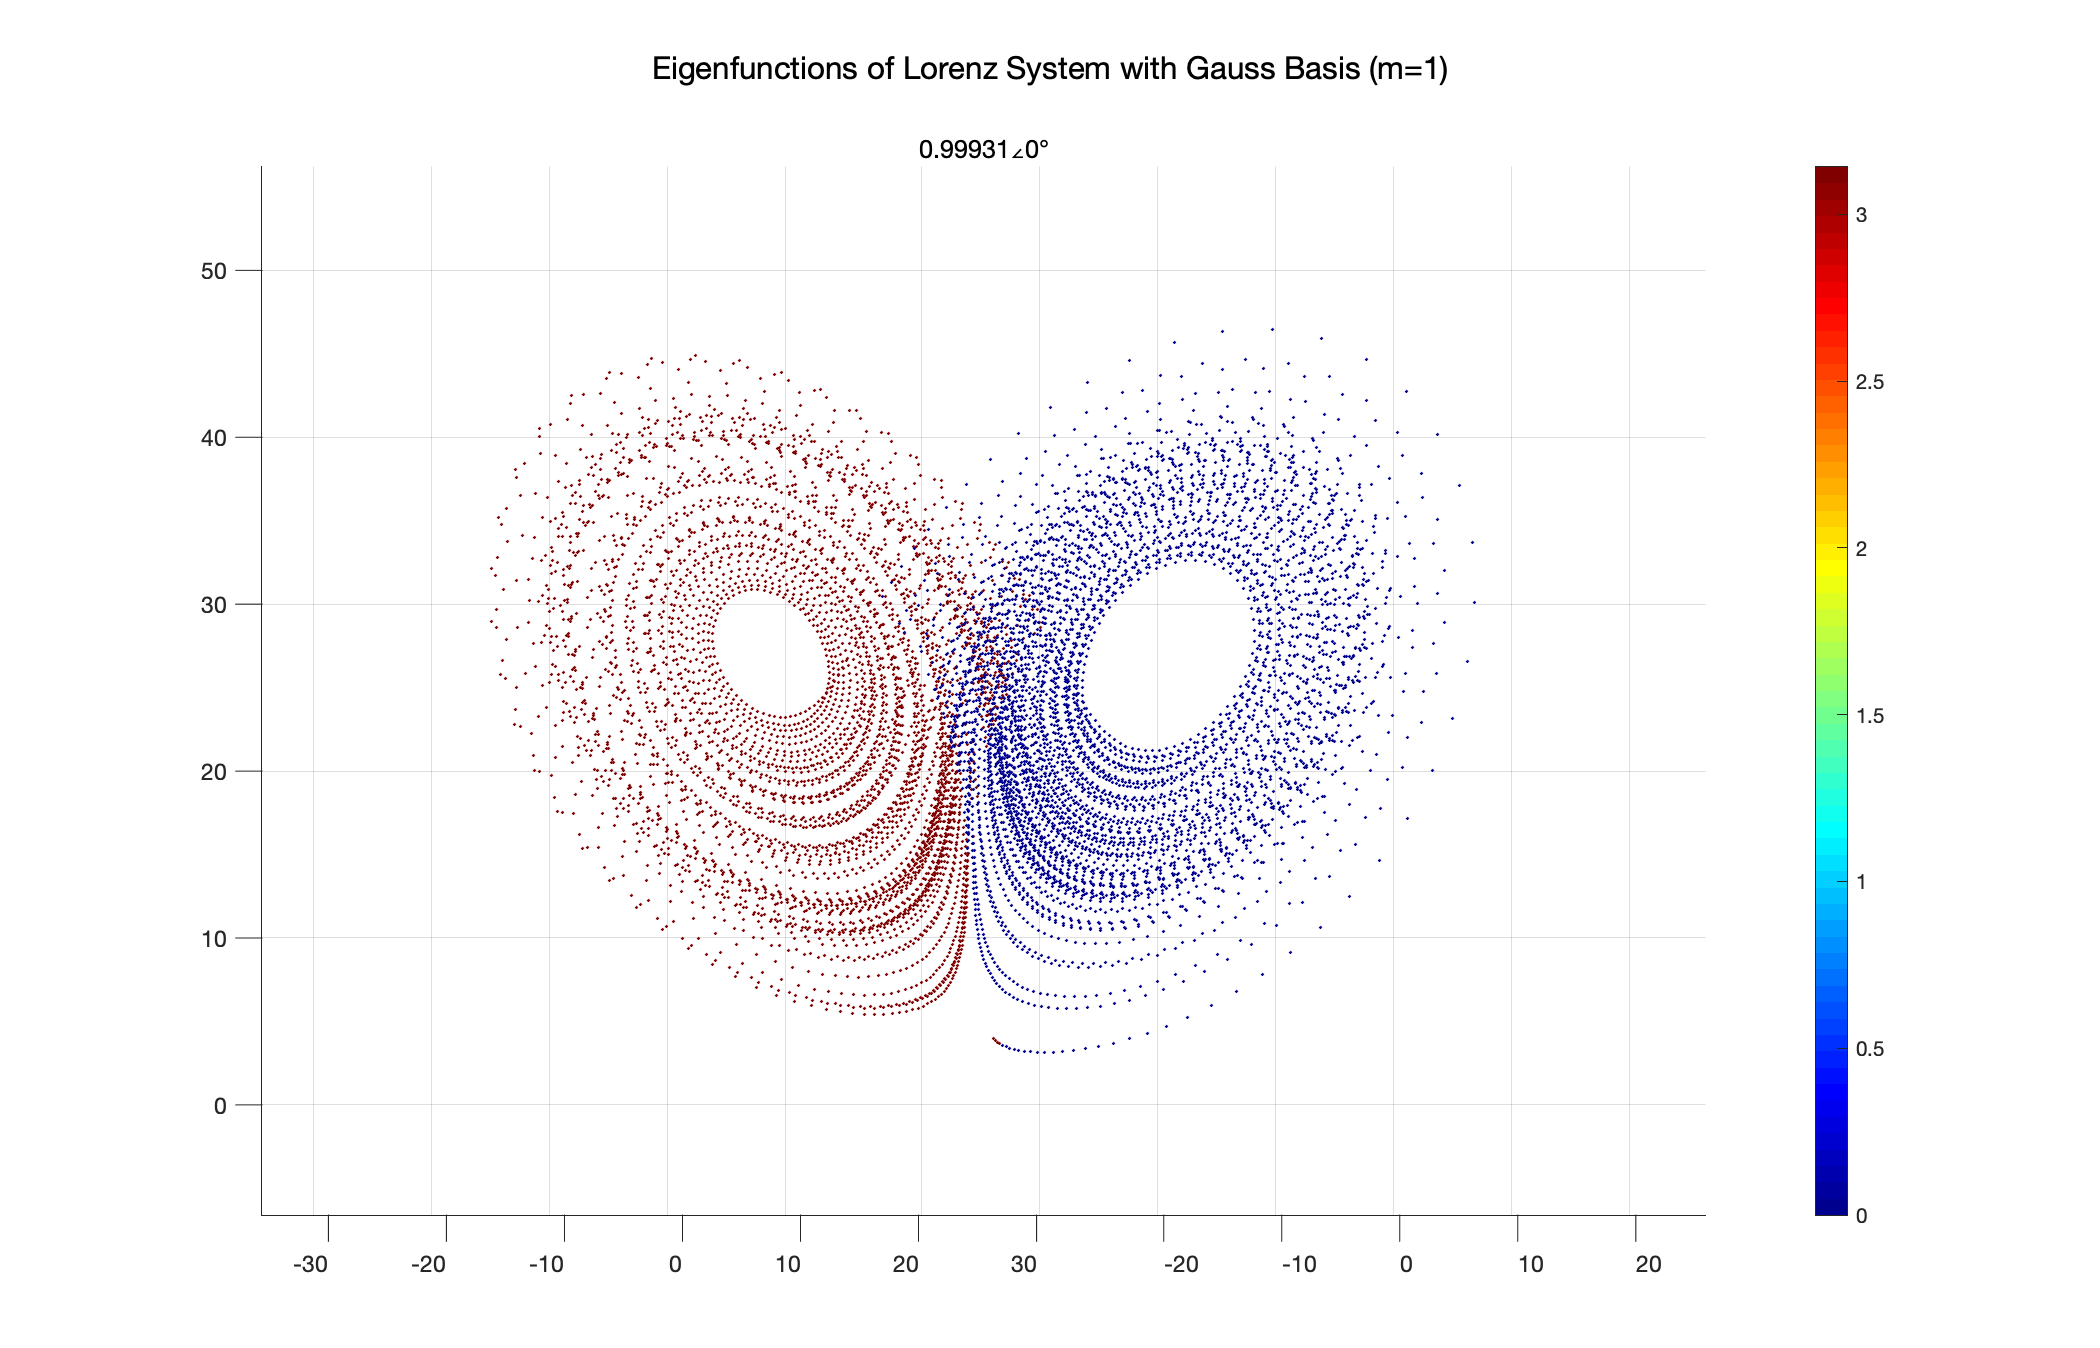
\includegraphics[scale=0.2]{lorenz/natural/multim/Lorenz_eigen_natural_multim_n10000m1dim1}}
    \subfloat[m=2]{
      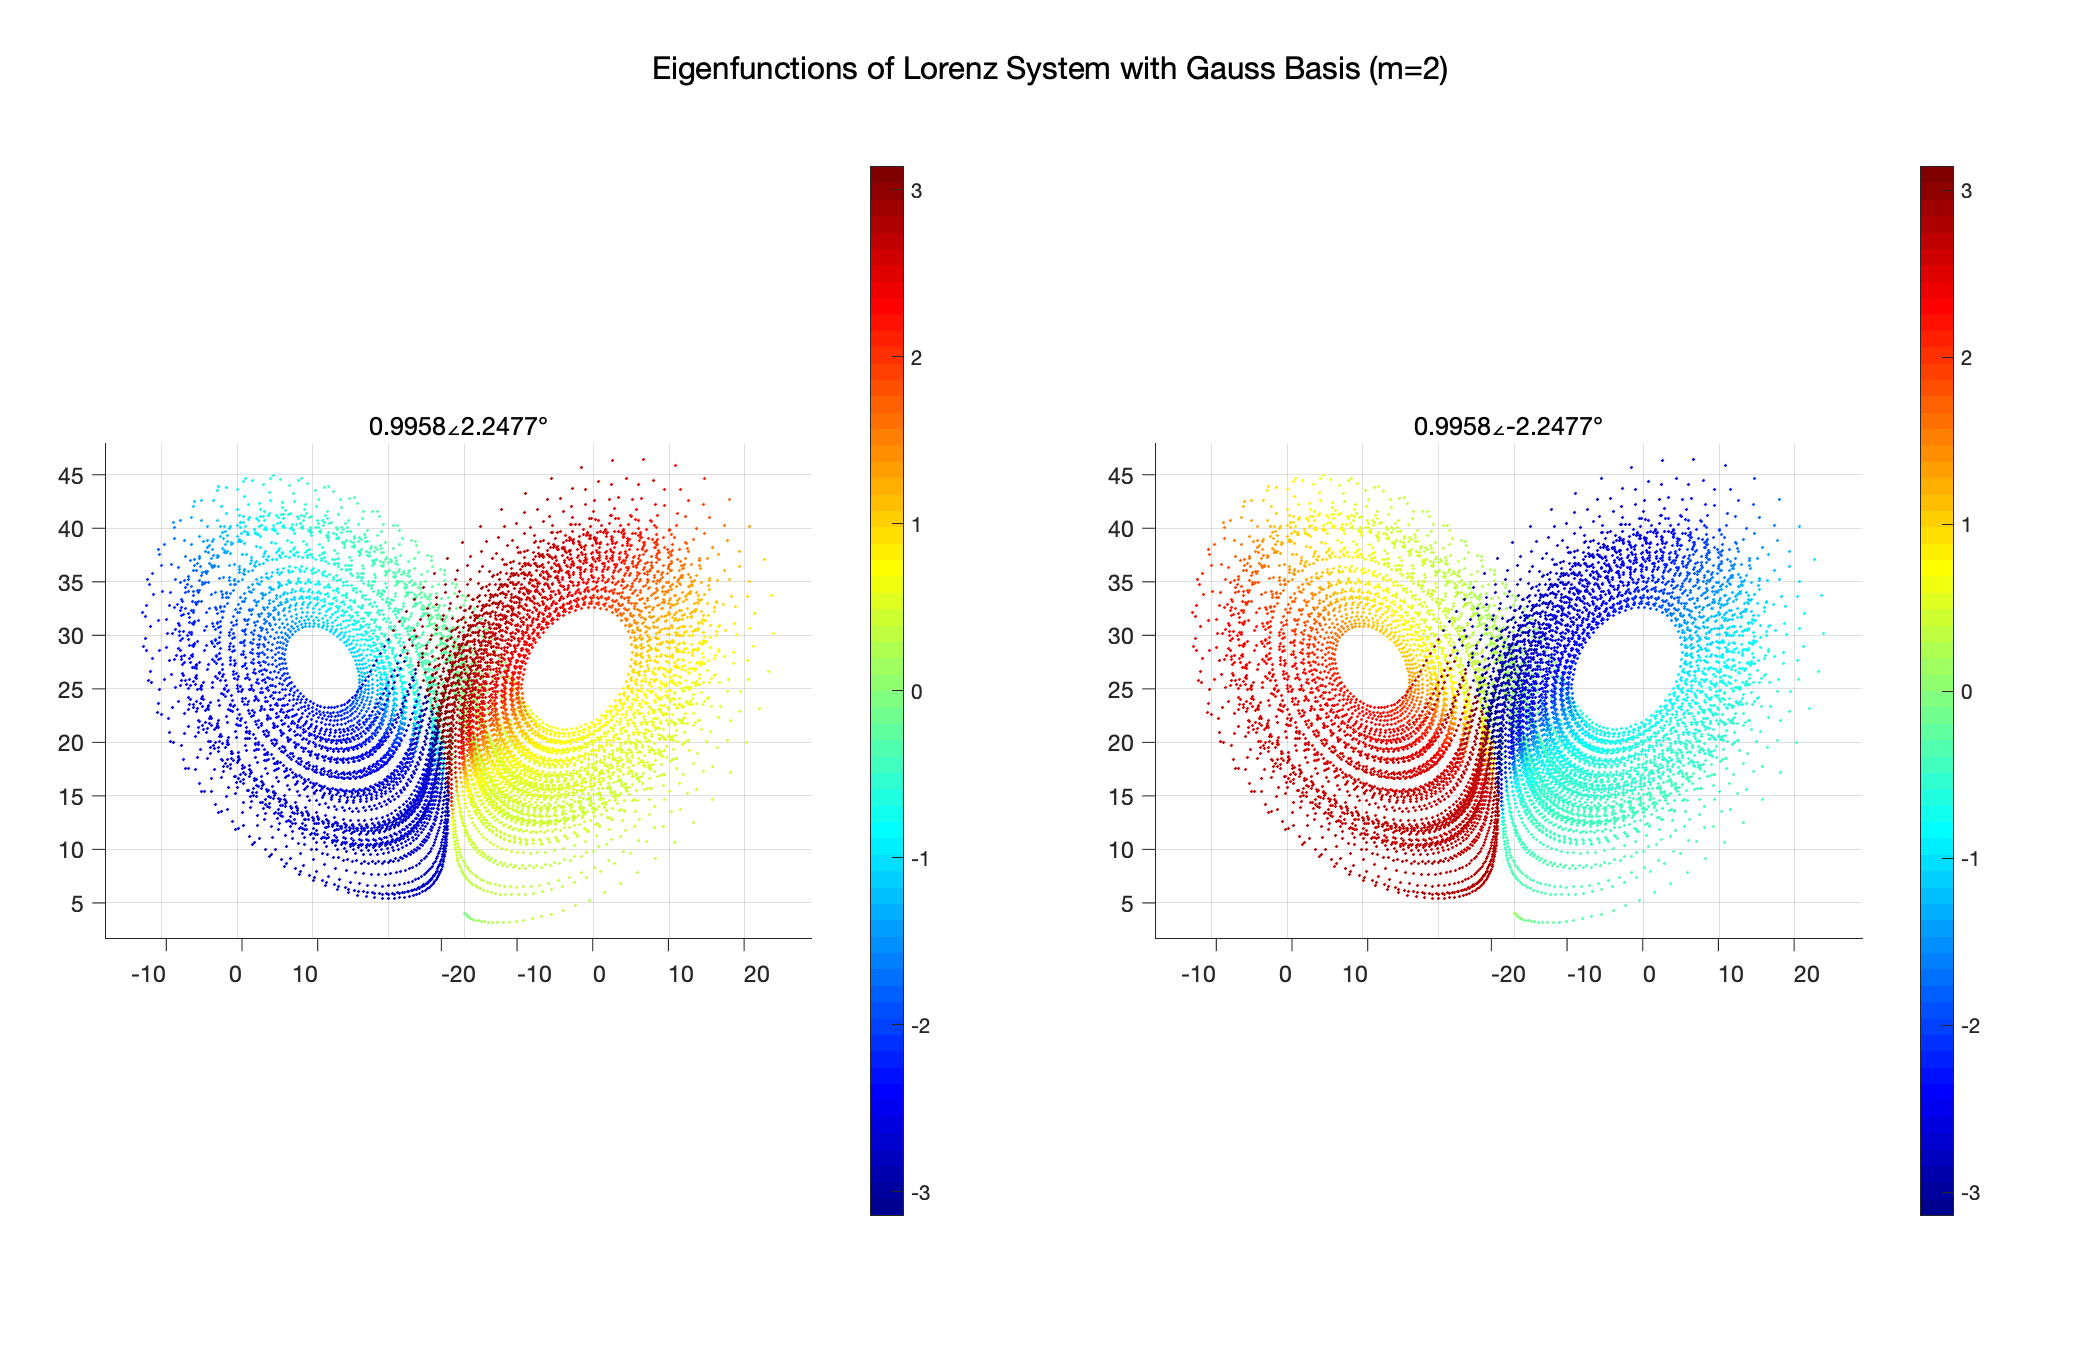
\includegraphics[scale=0.2]{lorenz/natural/multim/Lorenz_eigen_natural_multim_n10000m2dim1}}
    \\
    \subfloat[m=3]{
      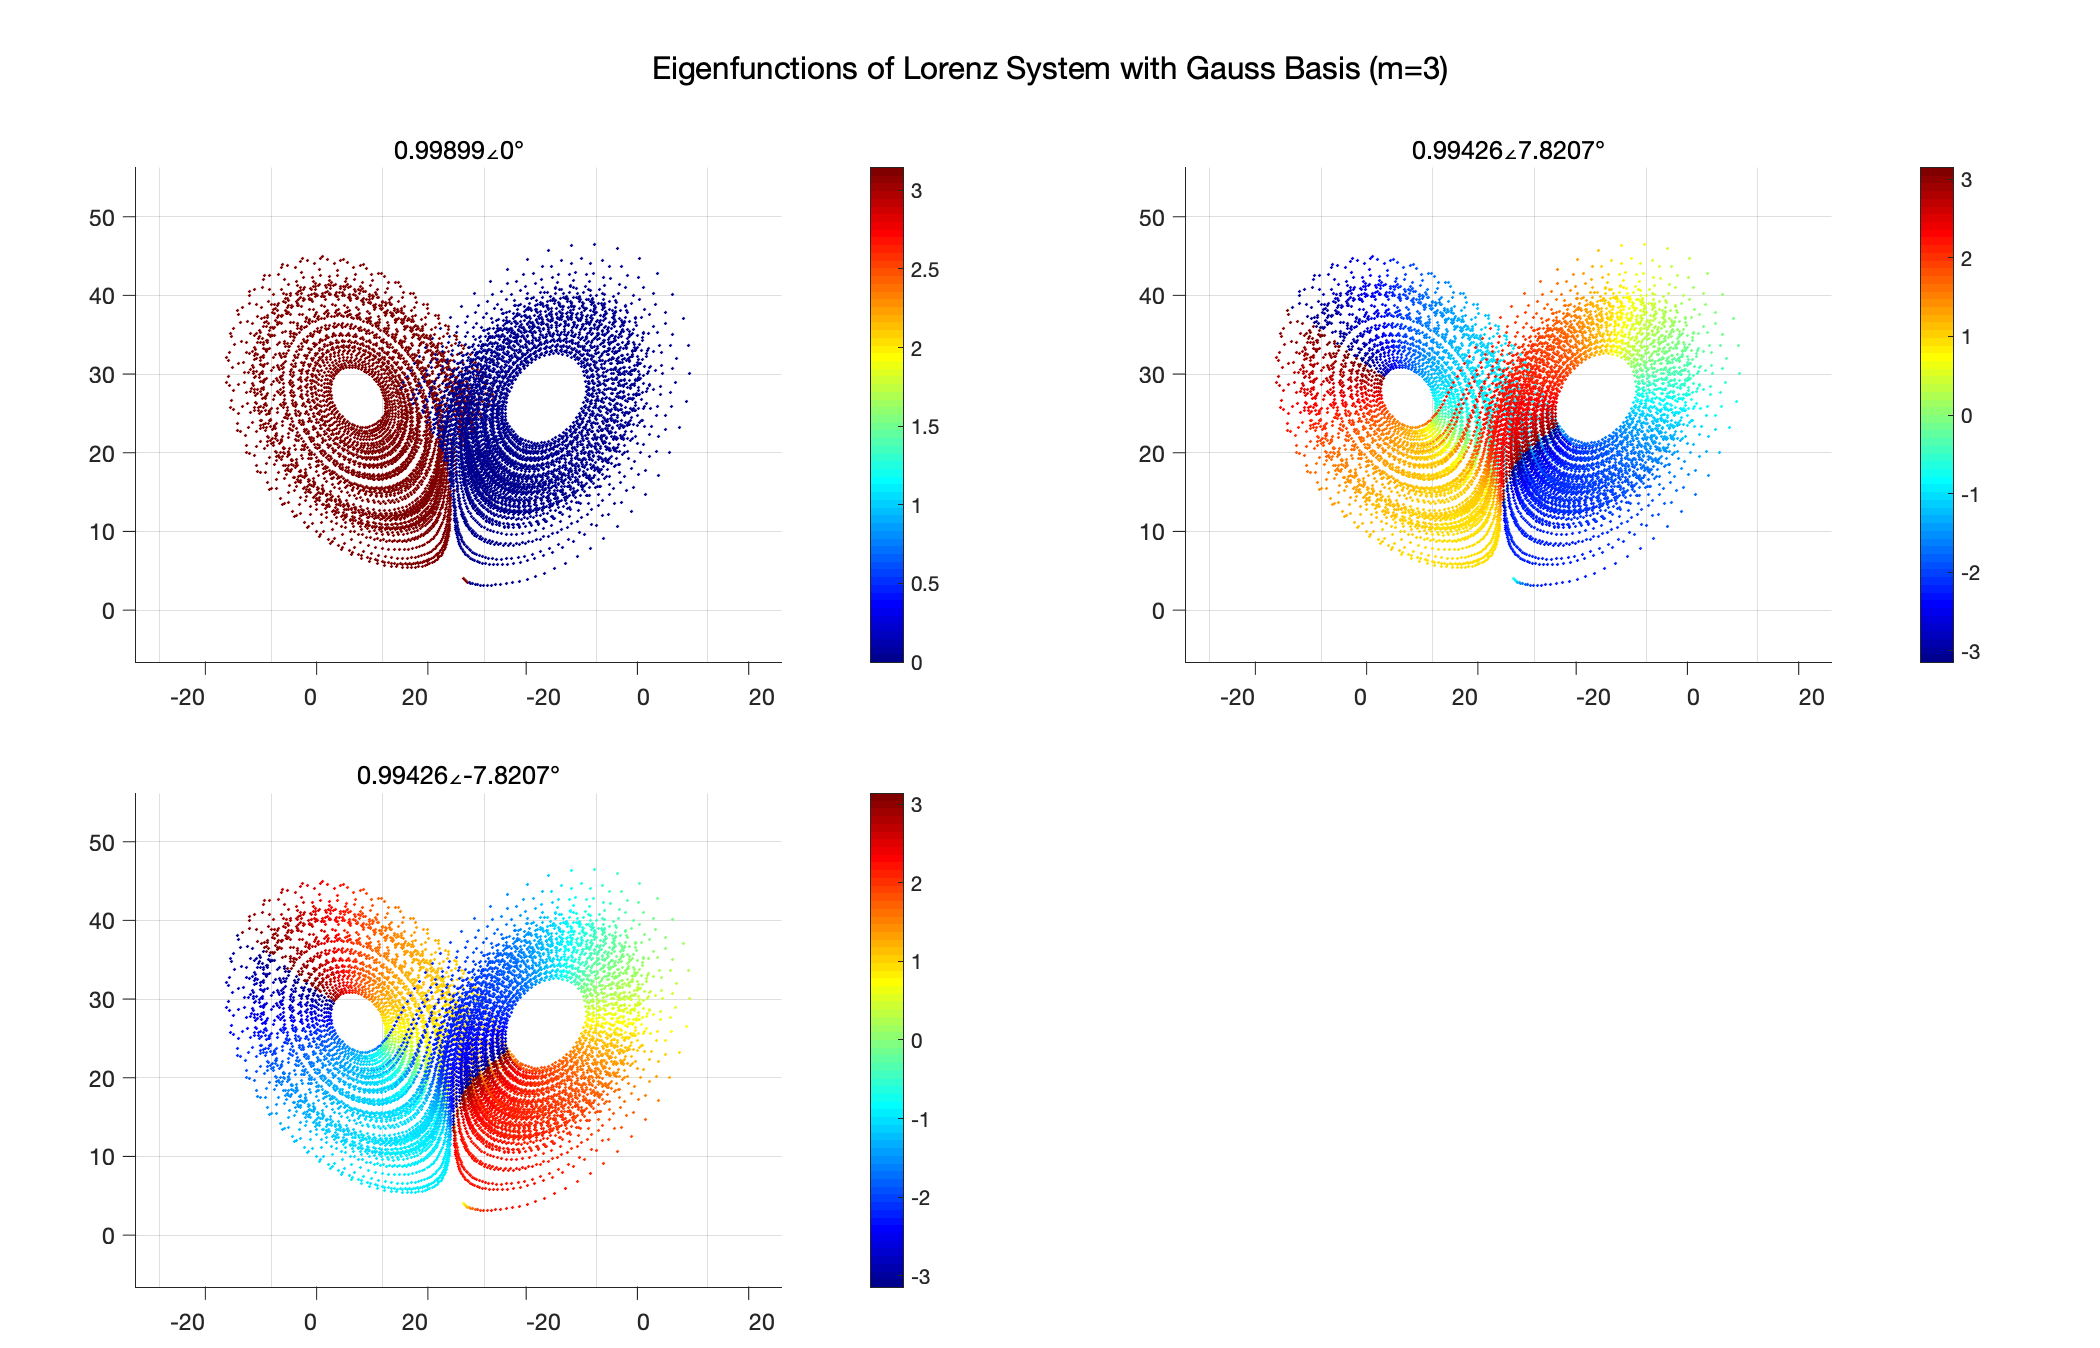
\includegraphics[scale=0.2]{lorenz/natural/multim/Lorenz_eigen_natural_multim_n10000m3dim1}}
    \subfloat[m=4]{
      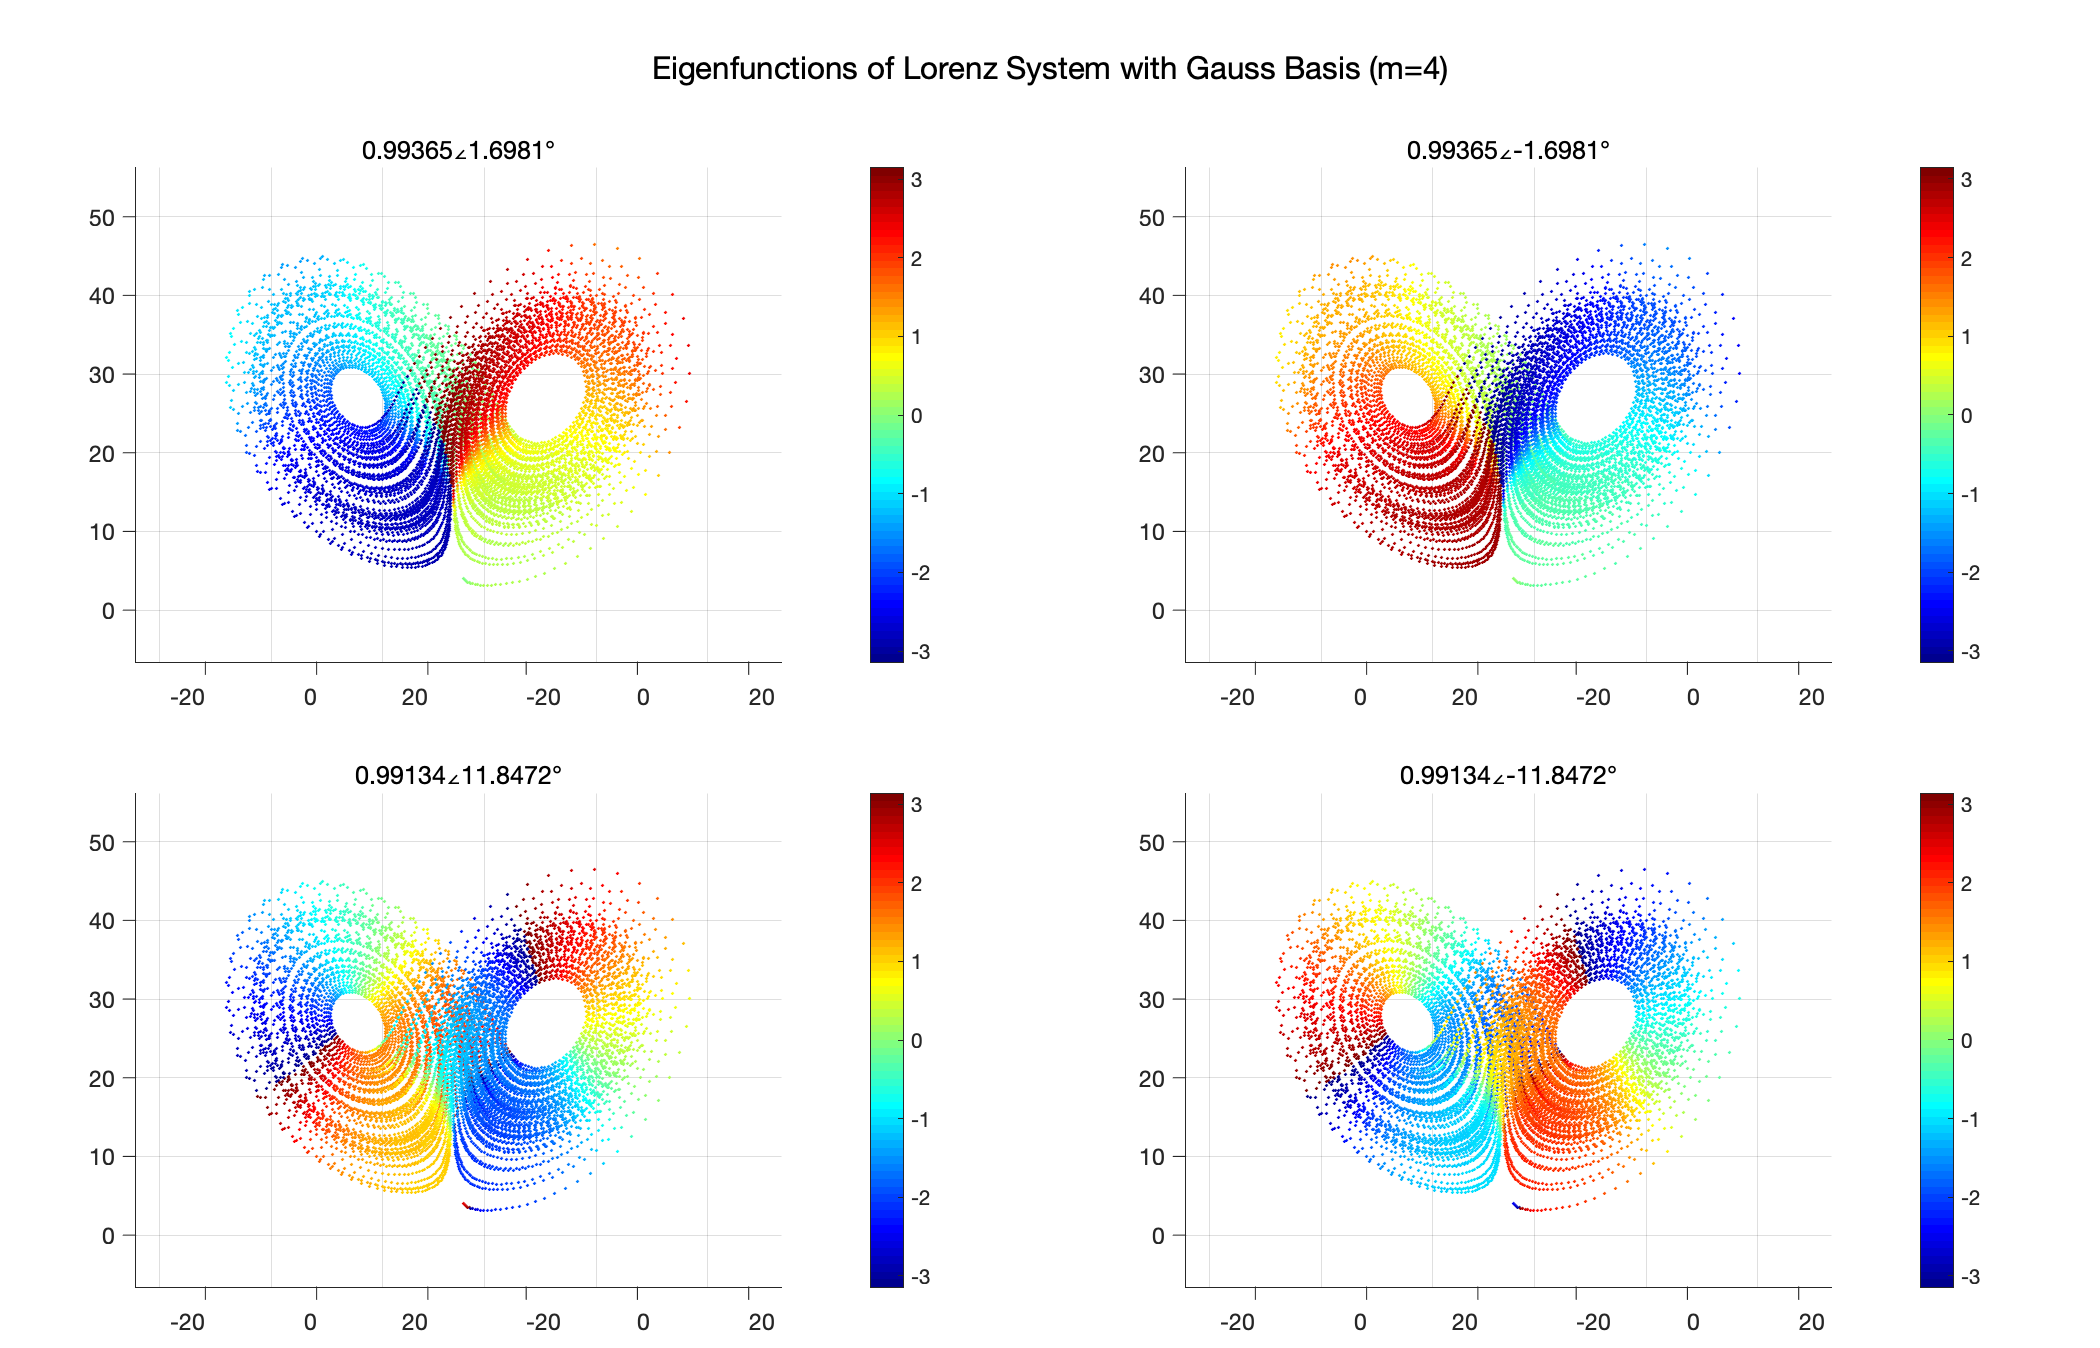
\includegraphics[scale=0.2]{lorenz/natural/multim/Lorenz_eigen_natural_multim_n10000m4dim1}}
    \\
    \subfloat[m=5]{
      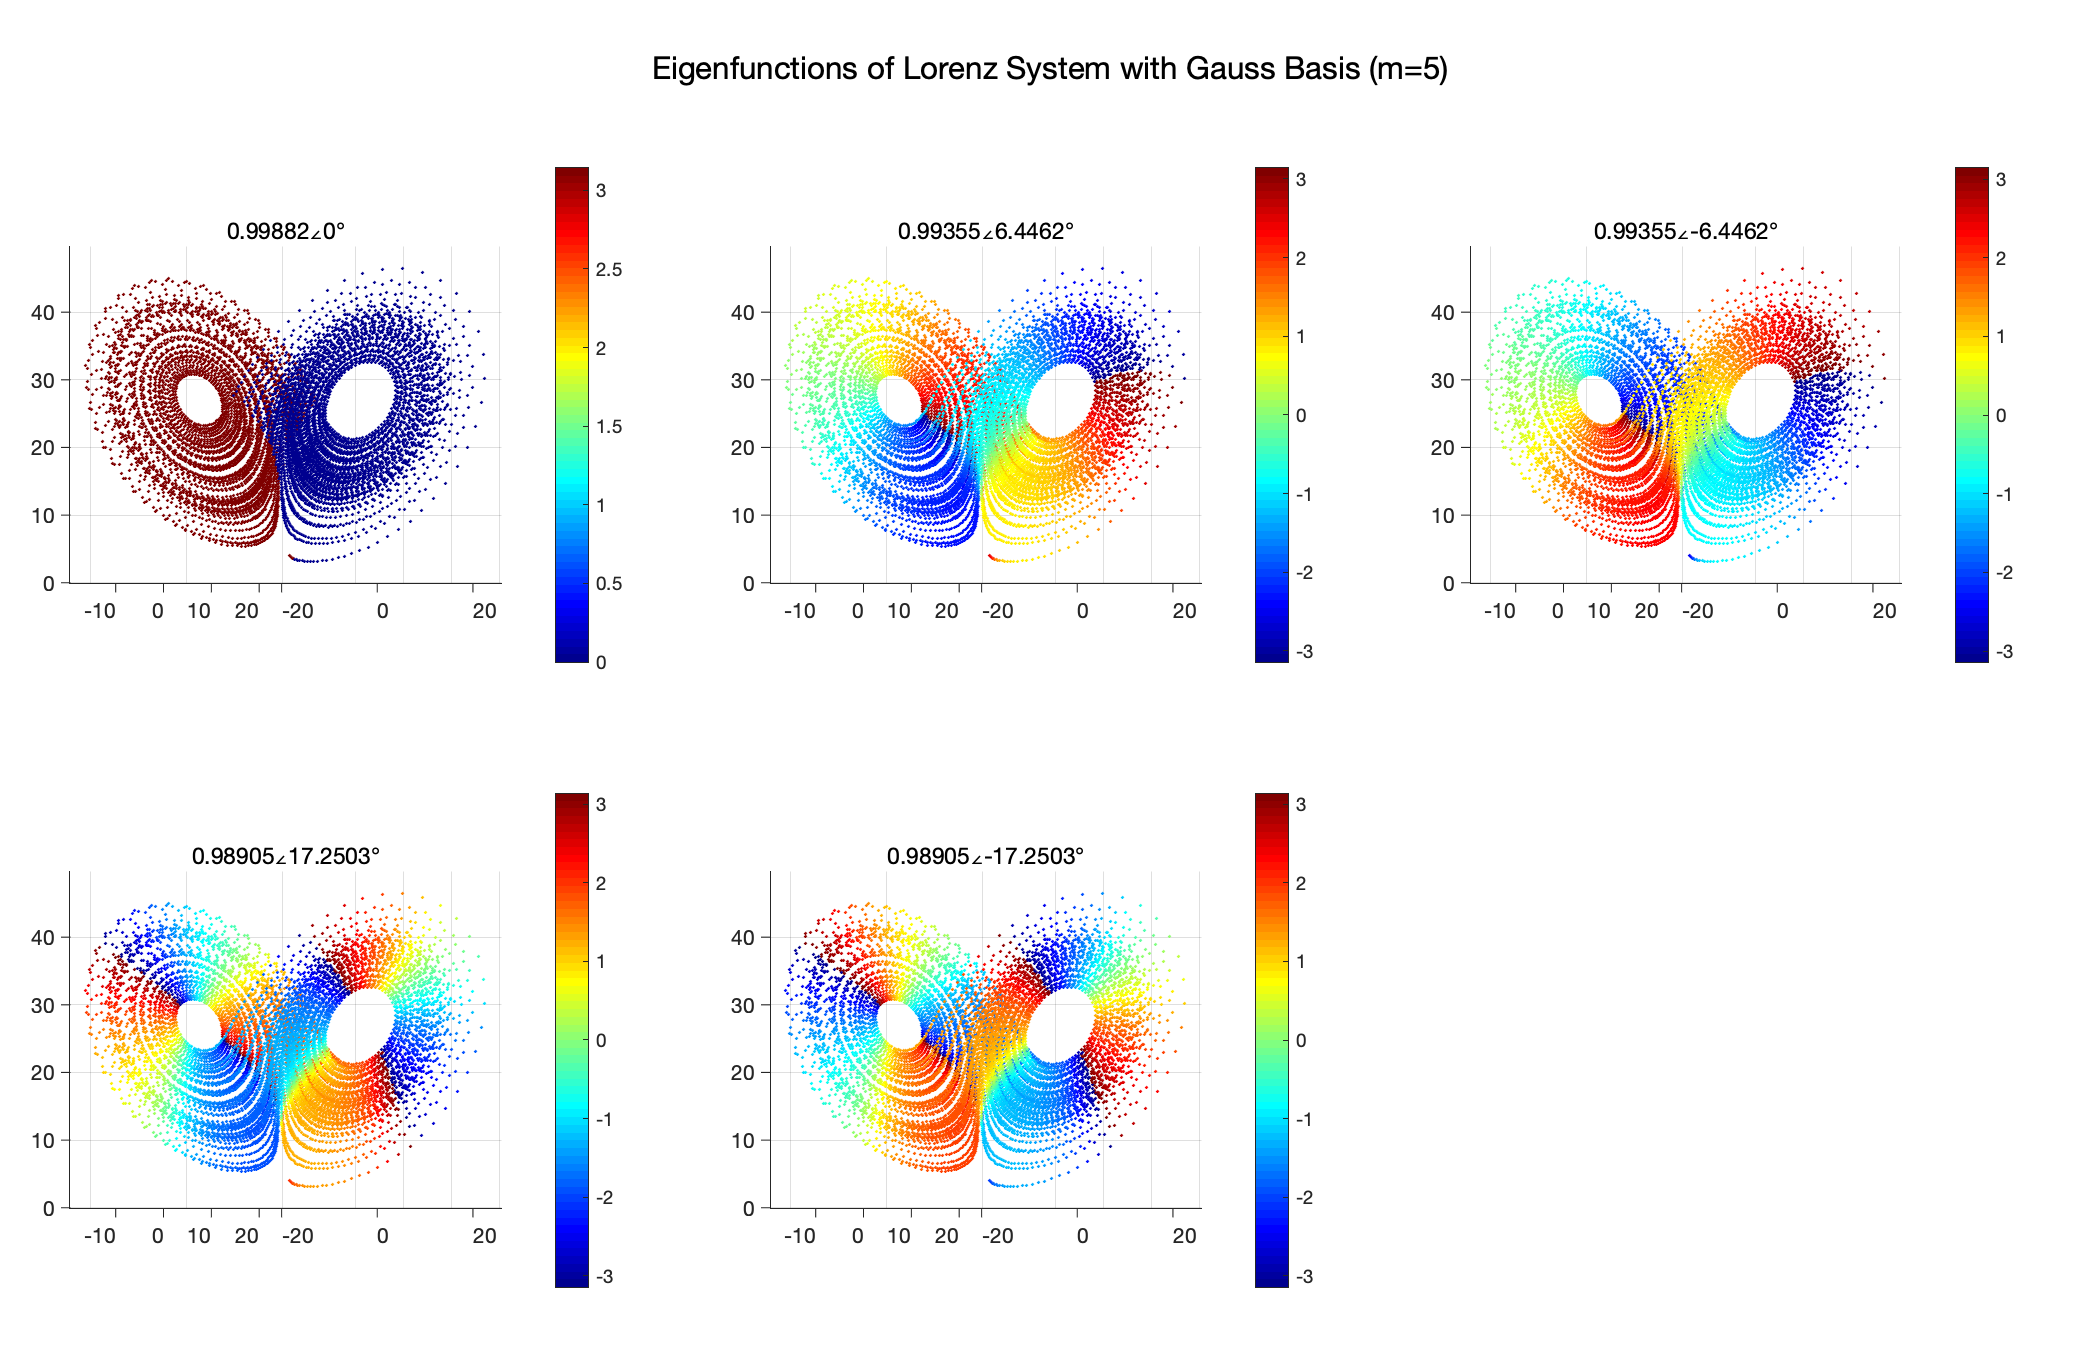
\includegraphics[scale=0.2]{lorenz/natural/multim/Lorenz_eigen_natural_multim_n10000m5dim1}}
    \subfloat[m=6]{
      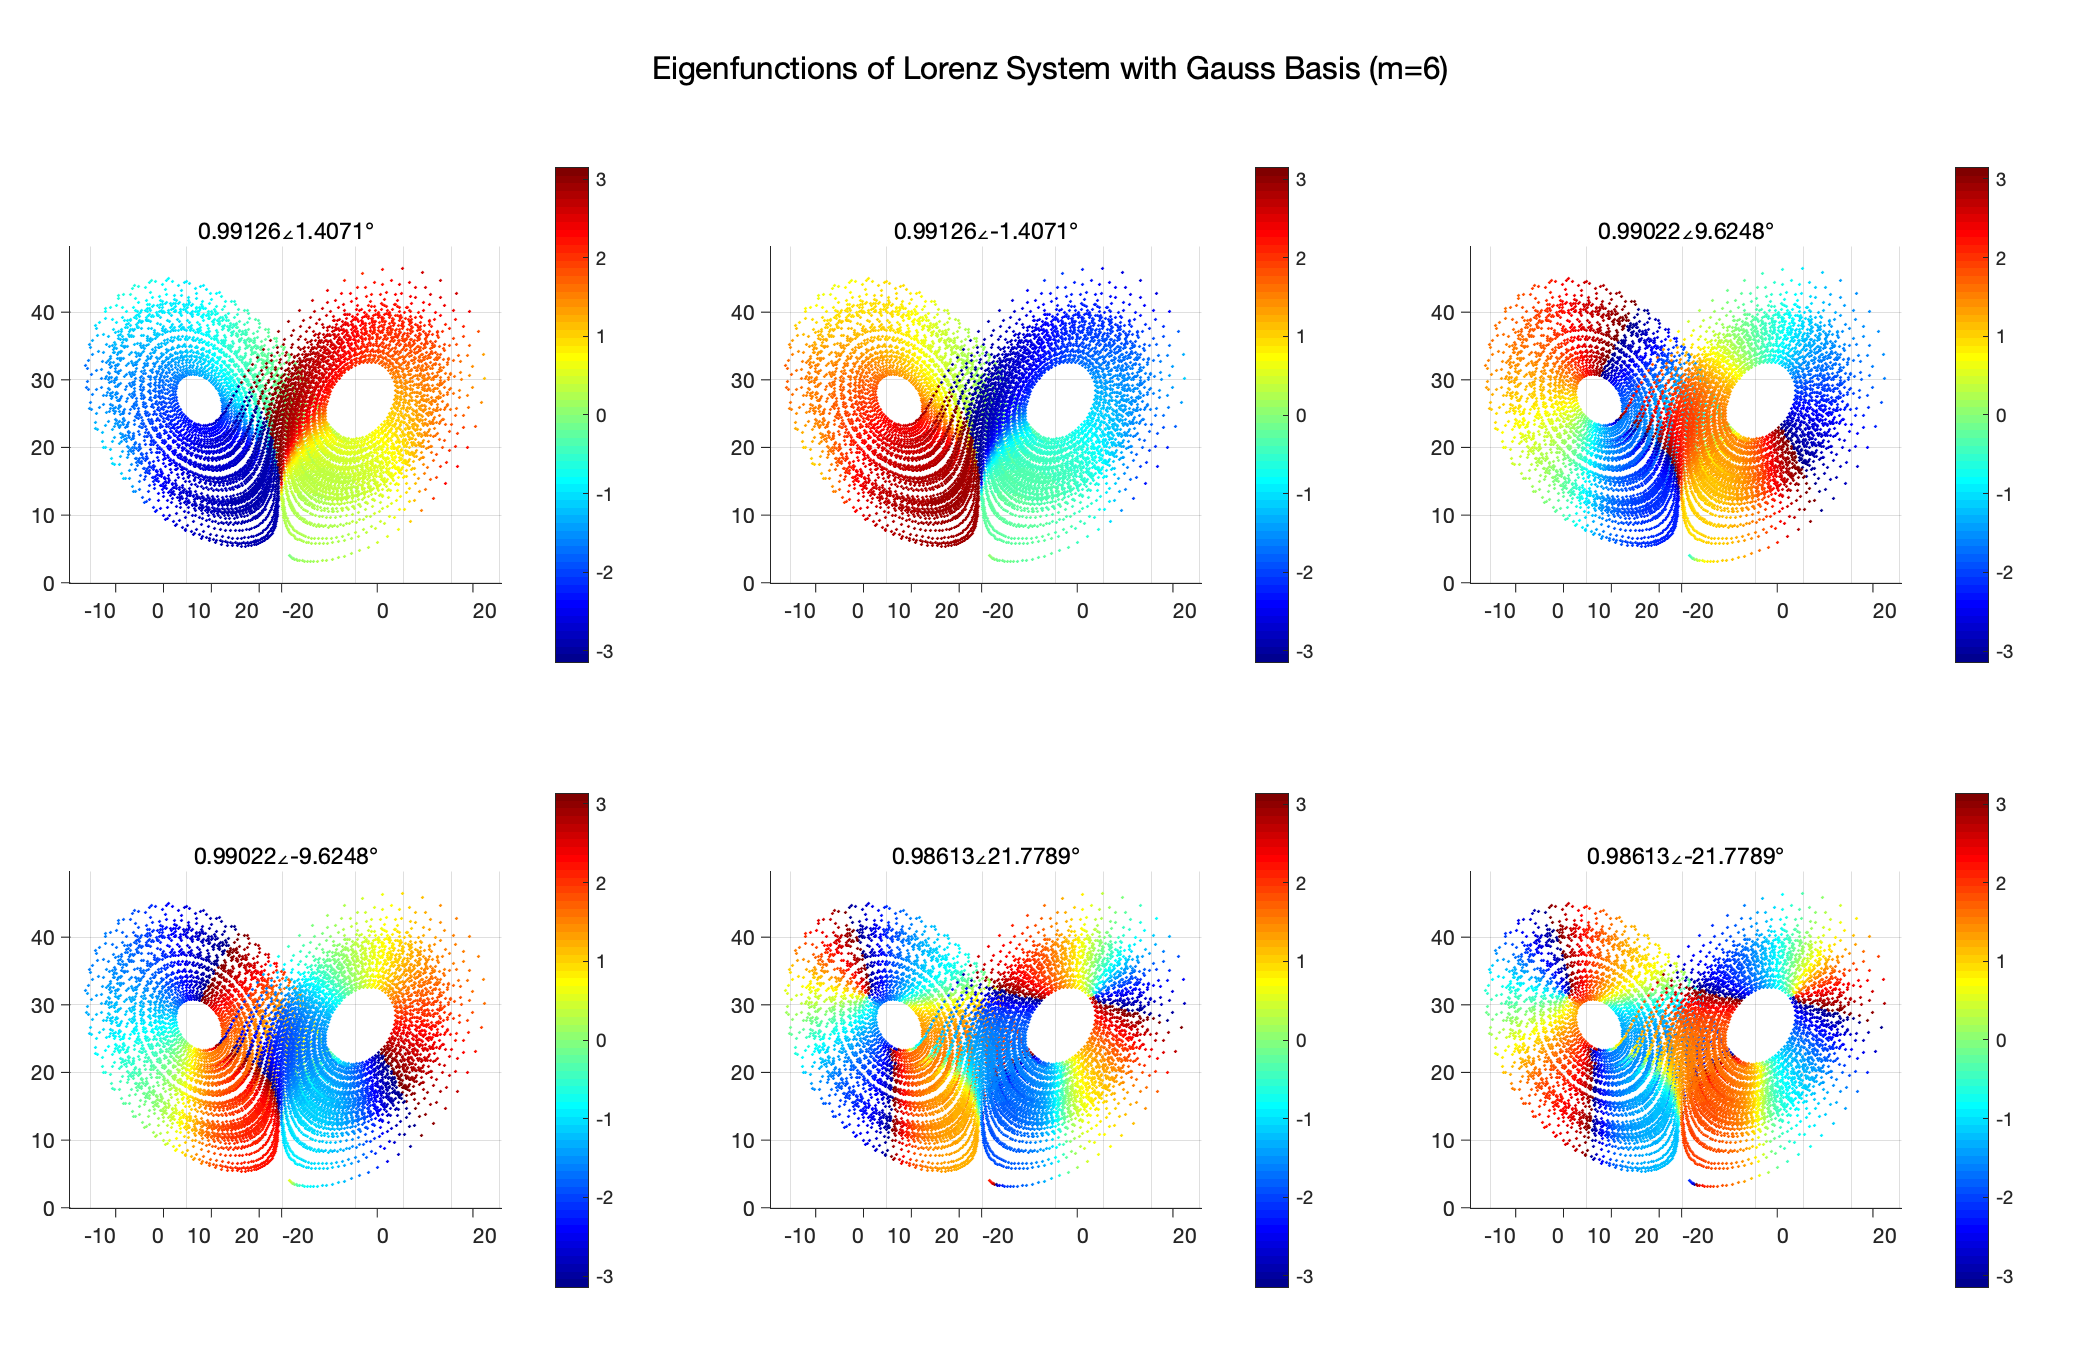
\includegraphics[scale=0.2]{lorenz/natural/multim/Lorenz_eigen_natural_multim_n10000m6dim1}}
    \\
    \subfloat[m=7]{
      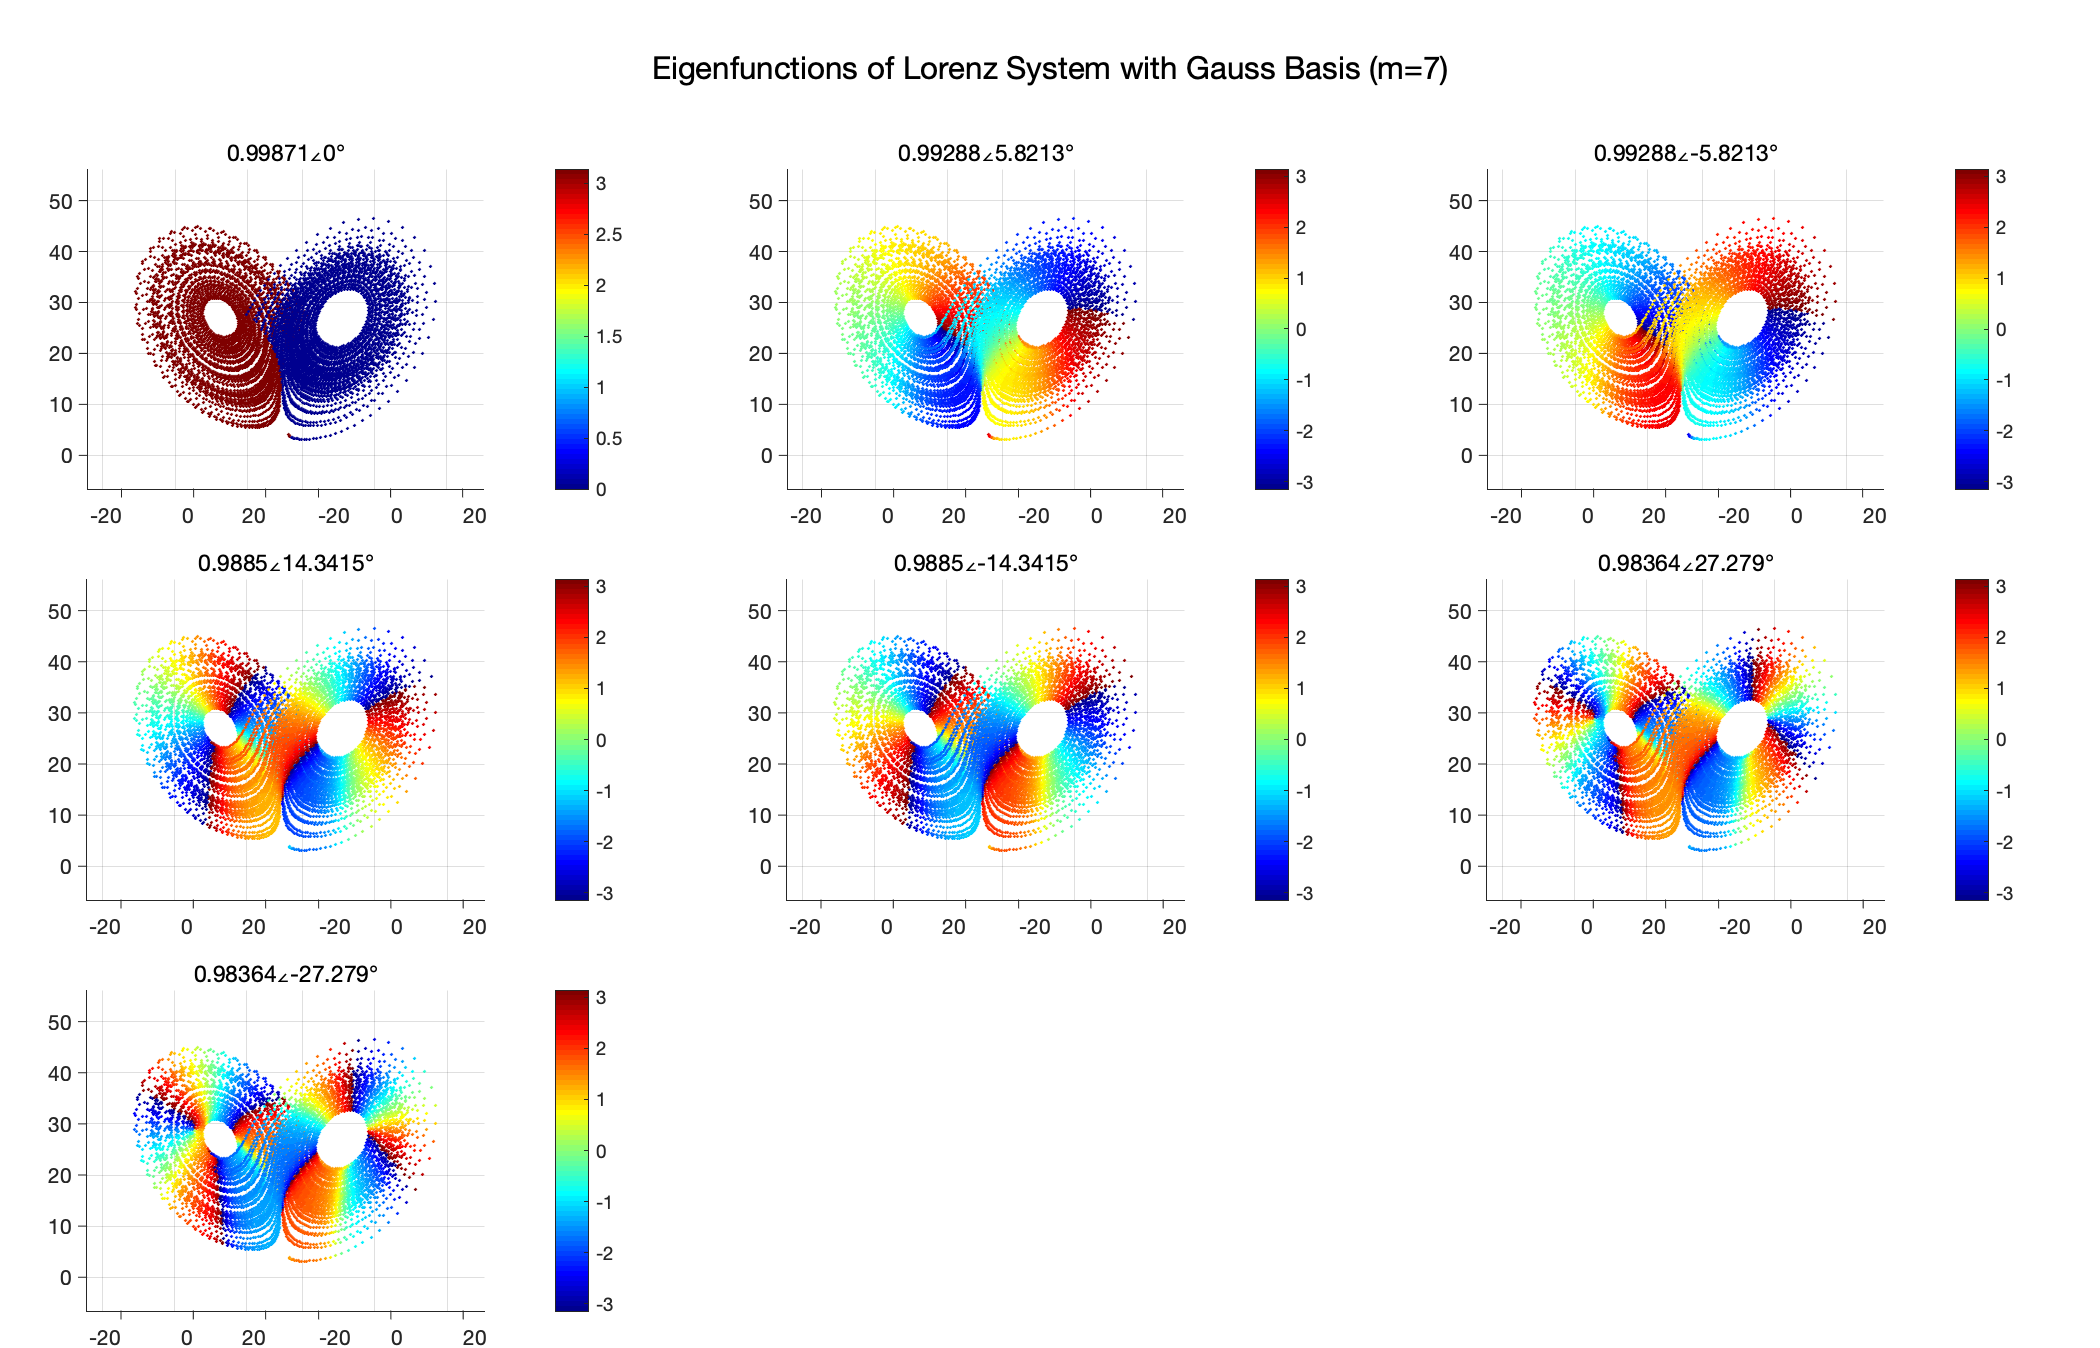
\includegraphics[scale=0.2]{lorenz/natural/multim/Lorenz_eigen_natural_multim_n10000m7dim1}}
    \subfloat[m=8]{
      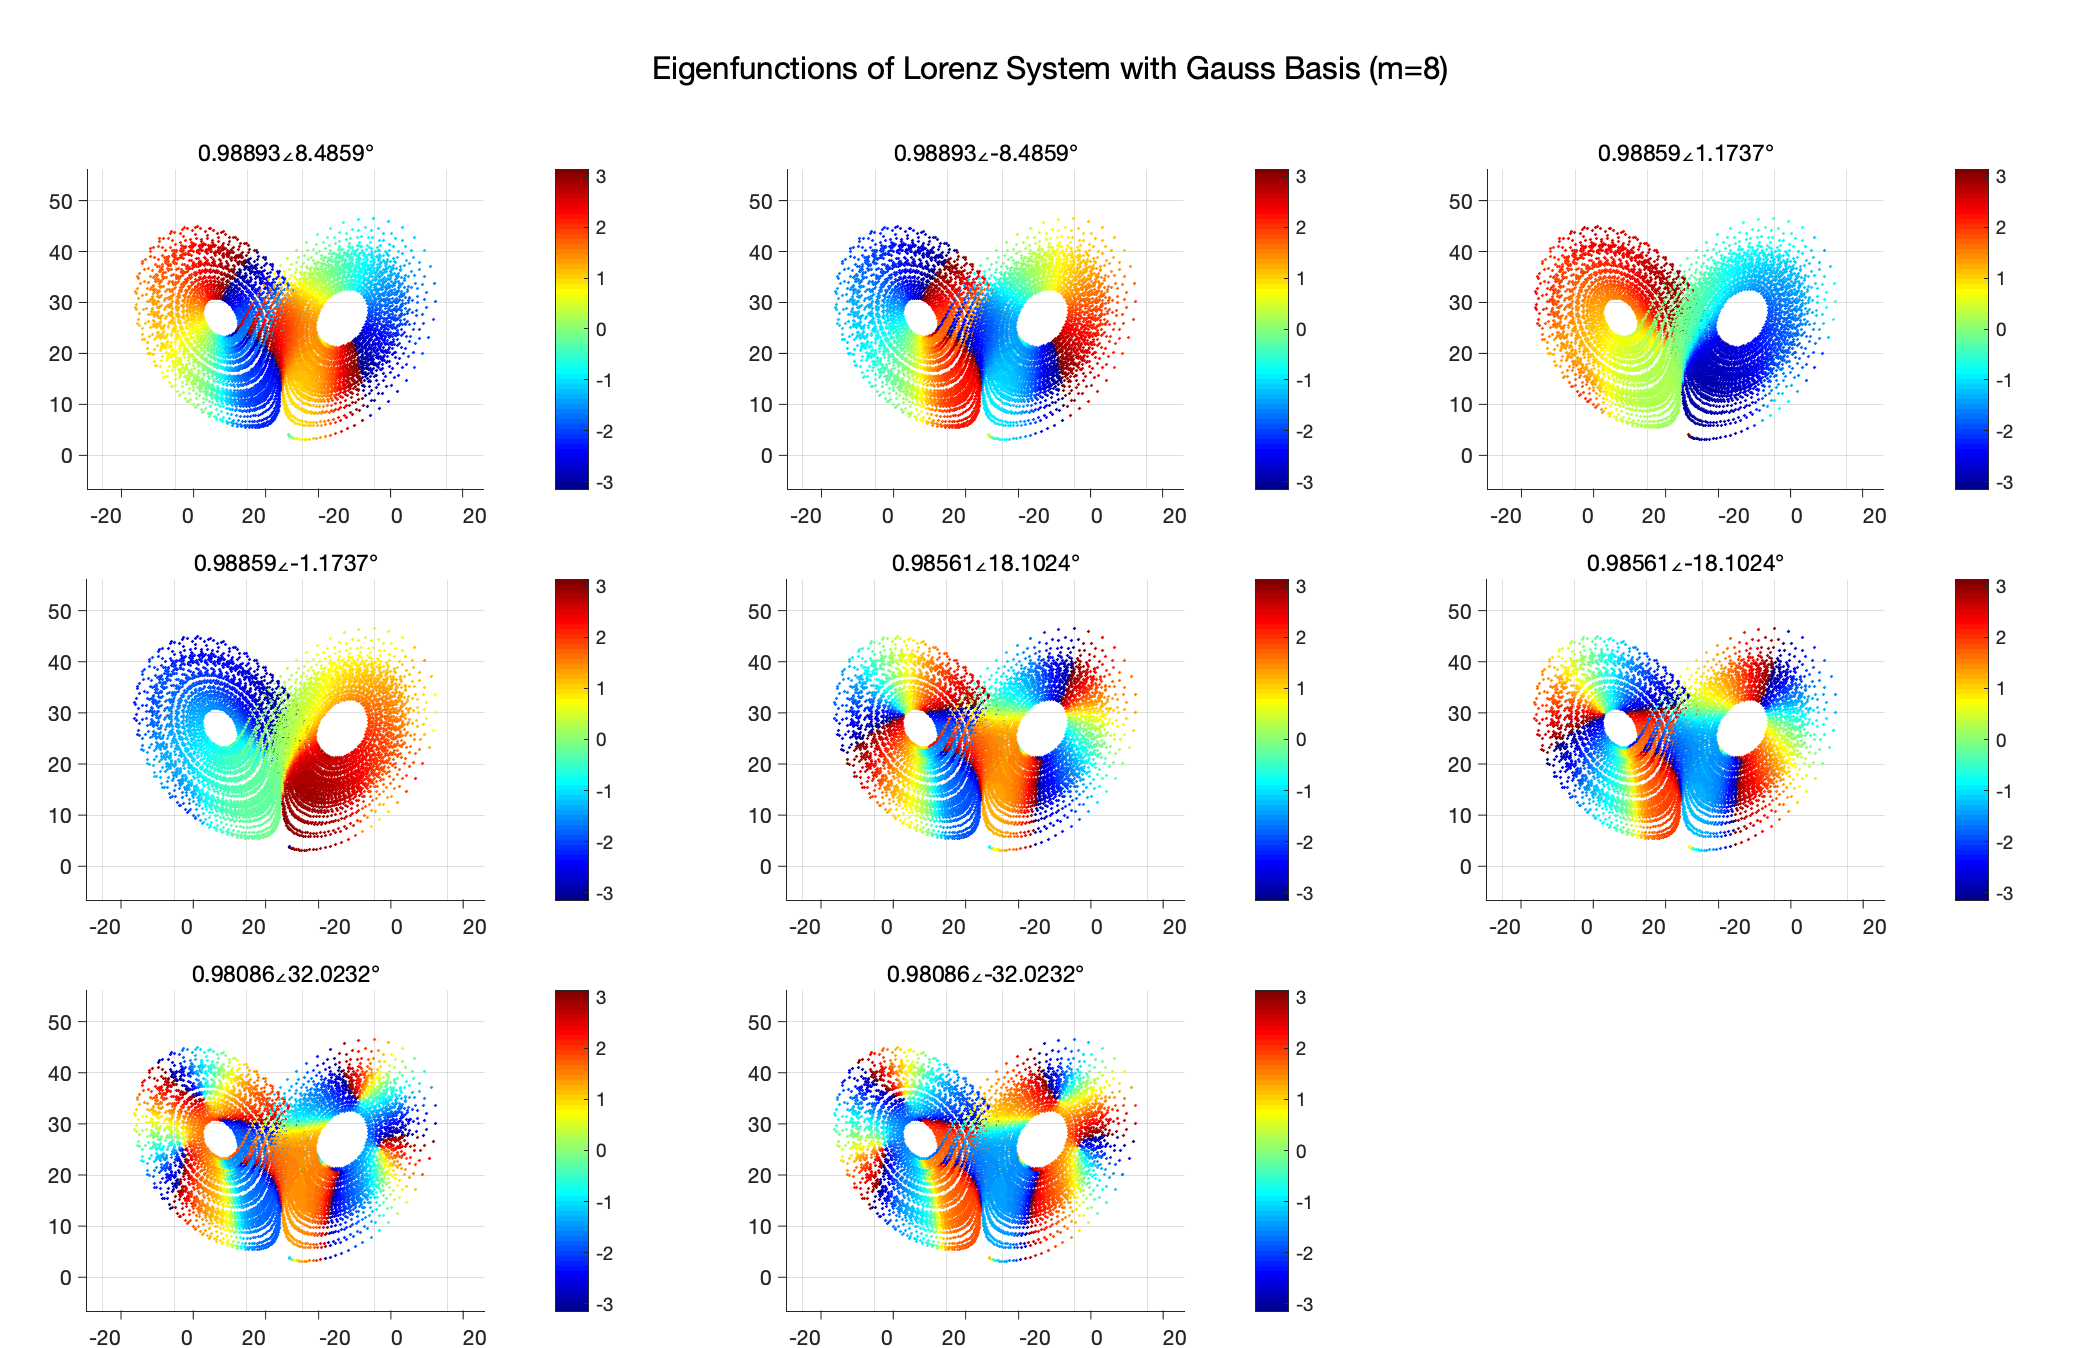
\includegraphics[scale=0.2]{lorenz/natural/multim/Lorenz_eigen_natural_multim_n10000m8dim1}}
    \\
    \caption{洛伦兹系统不同自然基函数数量下的real(x)本征函数($n=10000$)}\label{fig:lorenz_eig_natural_real}
\end{figure}

图\ref{fig:lorenz_eig_natural_real}中可以看出,随着基函数数量的增加,本征函数的数量也变得更多,吸引子上的倍频特征也越来越明显,如$m=1$时,不存在倍频特征,且本征函数将洛伦兹吸引子的左右两瓣划分为不同区域;当$m=2,3,4$时,本征函数在随着吸引子的演化中近似出现了一倍频;当$m=5,6$时,本征函数在随着吸引子的演化中近似出现了二倍频;当$m=7,8$时,本征函数在随着吸引子的演化中近似出现了三倍频。这个结论与低维映射中有一定一致性:随着基函数数量$m$的增加,相空间的一次演化$f$即体现一次变换,多次演化$f^n$就会体现多次变换,这种变换便对应了本征函数的倍频特征。若我们将这种变换与低维映射中拉伸折叠相对应起来,我们便可以得到与低维系统一致的结论。

\subsection{Koopman算符对洛伦兹系统的相空间划分}

在洛伦兹系统的本征函数图像中,在高斯基函数中,我们通过本征函数可以对相空间进行一定区域的划分,如使用本征函数的幅角正负可以将本征函数划分为两个区域,而这两个区域可以将吸引子划分为两个不变集,这两个不变化很可能与洛伦兹系统的周期轨道相对应,若我们根据本征函数值对吸引子划分,我们还可以得到更细致的划分,而这些划分是否能得到与低维系统一致的结论还需要进一步的讨论。

在自然基函数中,我们观察到本征函数的倍频特征,仅倍频数量随着基函数的增加而增加,基函数数量对应着自然基函数演化变换的次数,这种变化与低维映射中的拉伸折叠相对应,也可以得到和低维系统一致的结论。而关于Koopman算符对洛伦兹系统的相空间划分的验证则仍需要进一步的讨论。